%%%%%%%%%%%%%%%%%%%% author.tex %%%%%%%%%%%%%%%%%%%%%%%%%%%%%%%%%%%
%
% sample root file for your "contribution" to a contributed volume
%
% Use this file as a template for your own input.
%
%%%%%%%%%%%%%%%% Springer %%%%%%%%%%%%%%%%%%%%%%%%%%%%%%%%%%


% RECOMMENDED %%%%%%%%%%%%%%%%%%%%%%%%%%%%%%%%%%%%%%%%%%%%%%%%%%%
\documentclass[graybox]{svmult}

% choose options for [] as required from the list
% in the Reference Guide

\usepackage{mathptmx}       % selects Times Roman as basic font
\usepackage{helvet}         % selects Helvetica as sans-serif font
\usepackage{courier}        % selects Courier as typewriter font
\usepackage{type1cm}        % activate if the above 3 fonts are
                            % not available on your system
%
\usepackage{makeidx}         % allows index generation
\usepackage{graphicx}        % standard LaTeX graphics tool
                             % when including figure files
\usepackage{multicol}        % used for the two-column index
\usepackage[bottom]{footmisc}% places footnotes at page bottom

% see the list of further useful packages
% in the Reference Guide

\makeindex             % used for the subject index
                       % please use the style svind.ist with
                       % your makeindex program
\usepackage{amsmath}
\usepackage{amssymb}
\usepackage{siunitx} %SI notations looks nice

%%%%%%%%%%%%%%%%%%%%%%%%%%%%%%%%%%%%%%%%%%%%%%%%%%%%%%%%%%%%%%%%%%%%%%%%%%%%%%%%%%%%%%%%%
%% User dedined marcro 



\newcommand{\e}[2]{{\mathbb E}_{#1}\left[ #2 \right]}
\newcommand{\s}[2]{{\frac{1}{{#1}}\sum_{n=1}^{#1}} {#2}}
\newcommand{\q}[2]{{\mathcal Q}_{#1}\left( #2 \right)}
\newcommand{\p}{\mathbb P}
\newcommand{\sub}[1]{_{\text{#1}}}
\newcommand{\supe}[1]{^{\text{#1}}}
\newcommand{\pd}{\text{P}\sub{d}}
\newcommand{\pdac}{{\text{P}}\sub{d}\supe{}}
\newcommand{\pdoc}{{\text{P}}\sub{d}\supe{}}
\newcommand{\pfa}{\text{P}\sub{fa}}
\newcommand{\pfaac}{{\text{P}}\sub{fa}\supe{}}
\newcommand{\pfaoc}{{\text{P}}\sub{fa}\supe{}}
\newcommand{\phz}{\p(\mathcal{H}_0)}
\newcommand{\pho}{\p(\mathcal{H}_1)}
\newcommand{\pc}{\text{P}\sub{c}}
\newcommand{\pcd}{\bar{\text{P}}\sub{c}}
\newcommand{\pdd}{\bar{\text{P}}\sub{d}}

\newcommand{\prcvd}{P\sub{Rx,ST}}
\newcommand{\prcvdsr}{P\sub{Rx,SR}}
\newcommand{\eprcvd}{\hat{P}\sub{Rx,ST}}
\newcommand{\eprcvdsr}{\hat{P}\sub{Rx,SR}}
\newcommand{\bprcvd}{{P}\sub{Rx,ST}}
\newcommand{\ptranst}{P\sub{Tx,ST}}
\newcommand{\ptranpt}{P\sub{Tx,PT}}

\newcommand{\yrcvd}{y\sub{ST}}
\newcommand{\pp}{P\sub{p}}
\newcommand{\bpp}{\bar{P}\sub{p}}
\newcommand{\xp}{x\sub{PT}}
\newcommand{\xs}{x\sub{ST}}
\newcommand{\ps}{P\sub{s}}
\newcommand{\ys}{y\sub{SR}}
\newcommand{\ls}{\lambda\sub{}}
\newcommand{\Ks}{N\sub{s}}
\newcommand{\lp}{\lambda\sub{p}}
\newcommand{\Kp}{N\sub{p,2}}

\newcommand{\ap}{a\sub{2}}
\newcommand{\bp}{b\sub{2}}
\newcommand{\as}{a\sub{1}}
\newcommand{\bs}{b\sub{1}}


\newcommand{\rs}{R\sub{s}}
\newcommand{\rsac}{R\sub{s}\supe{AC}}
\newcommand{\rsoc}{R\sub{s}\supe{OC}}
\newcommand{\trs}{{R}\sub{s}}
\newcommand{\trsac}{{R}\sub{s}\supe{}}
\newcommand{\trsoc}{{R}\sub{s}\supe{}}
\newcommand{\ers}{\e{}{\rs}}

\newcommand{\gp}{g\sub{p}}
\newcommand{\gpo}{g\sub{p,1}}
\newcommand{\gpt}{g\sub{p,2}}
\newcommand{\gs}{g\sub{s}}
\newcommand{\hp}{h\sub{p}}
\newcommand{\hpo}{h\sub{p,1}}
\newcommand{\hpt}{h\sub{p,2}}
\newcommand{\hs}{h\sub{s}}
\newcommand{\phpo}{|h\sub{p,1}|^2}
\newcommand{\phpt}{|h\sub{p,2}|^2}
\newcommand{\phs}{|h\sub{s}|^2}
\newcommand{\ehs}{\hat{h}\sub{s}}
\newcommand{\npo}{\sigma^2_{w}}
\newcommand{\spo}{\sigma^2_{x}}
\newcommand{\evar}{\frac{\npo}{2 \Ks}}
\newcommand{\fsam}{f\sub{s}}

\newcommand{\ttau}{\tilde{\tau}}
\newcommand{\test}{\tau\sub{est}}
\newcommand{\ttest}{\tilde{\tau}\sub{est}}
\newcommand{\tsen}{\tau\sub{sen}}
\newcommand{\ttsen}{\tilde{\tau}\sub{sen}}
\newcommand{\ttsenac}{\tilde{\tau}\sub{sen}\supe{}}
\newcommand{\ttsenoc}{\tilde{\tau}\sub{sen}\supe{}}

\newcommand{\cz}{\text{C}_0}
\newcommand{\co}{\text{C}_1}

%\newcommand{\mpd}{\mu\sub{$\pd$}}
\newcommand{\mpd}{\kappa}

\newcommand{\snrp}{\frac{\ptranpt}{\npo}}
\newcommand{\snrs}{\frac{\ptranst}{\npo}}
\newcommand{\snrsi}{\frac{\npo}{\ptranst}}
\newcommand{\snrst}{\frac{\ps}{\sigma^2}}
\newcommand{\snrrcvd}{{\gamma}\sub{p,1}}
\newcommand{\snrso}{{\gamma}\sub{s}}
\newcommand{\snrpt}{{\gamma}\sub{p,2}}

\newcommand{\snrsp}{\frac{|\ehs|^2 \ptranst}{\npo}\Big /\frac{\eprcvdsr}{\npo}}
\newcommand{\lambdas}{\frac{\sigma_w^4}{ 2 \Ks \ptranst}}
\newcommand{\lambdasinv}{\frac{2 \Ks \ptranst}{\sigma_w^4}}


% distribution functions
\newcommand{\fpd}{F_{\pd}}
\newcommand{\feprcvd}{F_{\eprcvd}}
\newcommand{\fcz}{F_{\cz}}
\newcommand{\fco}{F_{\co}}

% density functions
\newcommand{\dpd}{f_{\pd}}
\newcommand{\dsnrs}{f_{\frac{ |\ehs|^2 \ptranst}{\npo}}}
\newcommand{\dsnrp}{f_{\frac{\eprcvdsr}{\npo}}}
\newcommand{\dsnrsp}{f_{\frac{|\ehs|^2 \ptranst}{\npo}\Big /\frac{\eprcvdsr}{\npo}}}
\newcommand{\dcz}{f_{\cz}}
\newcommand{\dco}{f_{\co}}
\newcommand{\deprcvd}{f_{\eprcvd}}

% threshold 
\newcommand{\thric}{\mu\sub{IC}}
\newcommand{\thrac}{\mu\supe{}}
\newcommand{\throc}{\mu\supe{}}

\newcommand{\imp}{\uline}
\newcommand{\ur}{\uuline}
\newcommand{\ns}{\uwave}
\newcommand{\ws}{\sout}
\newcommand{\fl}{\dashuline}
\newcommand{\un}{\dotuline}
\DeclareMathOperator*{\Pro}{Pr}
\DeclareMathOperator*{\argmaxi}{argmax}
\DeclareMathOperator*{\maxi}{max}
\DeclareMathOperator*{\expec}{\mathbb{E}}
\DeclareMathOperator*{\gthan}{\ge}
\DeclareMathOperator*{\eqto}{=}
\DeclareMathOperator*{\cosi}{ci}
\DeclareMathOperator*{\sini}{si}
\DeclareMathOperator*{\iGamma}{\text{inv}-\Gamma}
\DeclareMathOperator*{\cchi2}{\mathcal{X}^2}
\DeclareMathOperator*{\ncchi2}{\mathcal{X}_1^2}
\DeclareMathOperator*{\ts}{\text{T}(\textbf{y})}

\newtheorem{theorem}{Theorem}
\newtheorem{optimization}{Optimization}
\newtheorem{case}{Case}
\newtheorem{constraint}{Constraint}
\newtheorem{lemma}{Lemma}
\newtheorem{prop}{Proposition}
\newtheorem{remark}{Remark}
\newtheorem{coro}{Corollary}
\newtheorem{defi}{Definition}
 
\makeatletter
\if@twocolumn
	\newcommand{\figscale}{0.9 \columnwidth}
\else
	\newcommand{\figscale}{0.46 \columnwidth}
\fi
\makeatother


%% Use url and break them if they are too long for the page
\usepackage[hyphens]{url}
\usepackage[caption=false,font=footnotesize]{subfig} %% Plotting Subfigures
\usepackage{color,psfrag}  % Because most of matlab figures are generated with laprint that generates a .tex(with psfrag commands) and .eps
\usepackage{tikz}   % Drawing tool that overlaps on the plotted figures
\usetikzlibrary{trees}


\begin{document}

\title*{Performance Analysis of Cognitive Radio Systems from a Deployment Perspective}

%\titlerunning{Performance Analysis of Cognitive Radio Systems}

\authorrunning{Ankit Kaushik et al.}

% Use \titlerunning{Short Title} for an abbreviated version of
% your contribution title if the original one is too long
\author{Ankit Kaushik, Shree Krishna Sharma, Symeon Chatzinotas, Bj\"orn Ottersten and Friedrich K. Jondral}
% Use \authorrunning{Short Title} for an abbreviated version of
% your contribution title if the original one is too long
\institute{A. Kaushik, F. K. Jondral \at Communications Engineering Lab, Karlsruhe Institute of Technology, Karlsruhe, Germany, \email{{Ankit.Kaushik, Friedrich.Jondral}@kit.edu}
\and S. K. Sharma, S. Chatzinotas, B. Ottersten \at SnT - securityandtrust, University of Luxembourg, Luxembourg \email{{Shree.Sharma, Symeon.Chatzinotas, Bjorn.Ottersten}@uni.lu}
}
%
% Use the package "url.sty" to avoid
% problems with special characters
% used in your e-mail or web address
%
\maketitle


\begin{abstract}
%Cognitive radio is envisioned as one of the potential candidates that addresses the issue of spectrum scarcity. 
Knowledge of interacting channels is essential for characterizing the performance of a cognitive radio system in terms of interference power received by a primary receiver and throughput at a secondary receiver. Baseline models considered for the performance characterization assume perfect knowledge of the interacting channels. Recently, an analytical framework has been proposed that incorporates channel estimation and subsequently characterizes the performance of cognitive Interweave Systems (ISs). However, the analysis was pertained to the deterministic behaviour of the interacting channels. In this paper, we extend the characterization of the aforementioned framework to investigate the influence of channel fading on the performance of the IS. %In this regard, we derive the expressions of the primary interference and the secondary throughput, 
%, where the interacting channels are subject to Nakagami-$m$ fading. 
Our analysis indicate that an inappropriate choice of estimation time can severely degrade the performance of the IS in terms of achievable secondary throughput. %specially for scenarios with severe fading. 
\end{abstract}


%%%%%%%%%%%%%%%%%%%%%%%%%%%%%%%%%%%%%%%%%%%%%%%%%%%%%%%%%%%%%%%%%%%%%%%%%%%%%%%%%%%%%%%%%
\section{Introduction}
%%%%%%%%%%%%%%%%%%%%%%%%%%%%%%%%%%%%%%%%%%%%%%%%%%%%%%%%%%%%%%%%%%%%%%%%%%%%%%%%%%%%%%%%%
%\subsection{Background}
%Goldsmith \textit{et .al} \cite{Goldsmith09}
The static allocation of the existing spectrum is largely responsible for causing scarcity in the spectrum. Cognitive Radio (CR) communication is foreseen as one of the potential contenders that could resolve this scarcity by utilizing the allocated spectrum efficiently. The widely investigated CR paradigms can be classified as follows: interweave, underlay and overlay systems \cite{Goldsmith09}. Among these, Interweave Systems (ISs) are mostly preferred for theoretical analysis as well as for hardware implementations \cite{Kaushik13, Kaushik15_Dy}. The ISs depend on spectrum sensing to detect the presence of Primary User (PU) signals. Several techniques such as energy detection, matched filtering, cyclostationary and feature detection exist for detecting the PU signal \cite{Sharma15}. Due to low complexity and versatility towards unknown PU signals, energy detection has been extensively employed for characterizing the performance of the IS \cite{Tan08, Liang08, Sharkasi12, Pradhan15}. In this regard, this paper focuses on the performance analysis of the cognitive ISs that employ estimation of the interacting channels, where the channels are subject to channel fading. 

\subsection{Motivation and Related Work}
The performance of the IS can be characterized jointly in terms of interference (power) received at the Primary Receiver (PR) from the Secondary Transmitter (ST) and throughput achieved at the Secondary Receiver (SR). The interference at the PR depends on the detector's performance (depicted in terms of detection probability) employed at the ST. On the other side, false alarm probability largely contributes to the secondary throughput. Due to the employment of periodic sensing at the ST, the achievable secondary throughput is related to the sensing time. By operating at a desired detection probability, the interference at the PR can be regulated below a tolerance limit. Along with the secondary throughput, the false alarm and the detection probabilities depend on the sensing time. This relationship between the sensing time and the secondary throughput subject to a target detection probability has been investigated by Liang \textit{et. al.} \cite{Liang08} as a sensing-throughput tradeoff. More specifically, the sensing-throughput tradeoff can be utilized for determining a suitable sensing time at which the maximum secondary throughput is achieved by the IS. 

It is worth noticing the fact that the detector employed for carrying out sensing is sensitive to the variations that arise due to presence of thermal noise in the system and fading in the channel. In this context, the characterization of the detection probability that captures the aforementioned variations has been carried out in the literature \cite{Kostylev02, Alouini03, Herath09}. Furthermore, Cardenas-Juarez \textit{et. al.} \cite{Juarez11} investigated the performance of the IS in terms of a sensing-throughput tradeoff. However, it is important to note that the performance analysis according to \cite{Alouini03, Herath09, Juarez11} assumes the perfect knowledge of the following interacting channels: \textit{sensing} channel for the link PT-ST, \textit{access} channel for the link ST-SR and \textit{interference} channel for the link PT-ST, refer to \figurename~\ref{fig:scenario}. From a deployment perspective, this knowledge is not available at the ST. In this context, an analytical framework that employs channel estimation at the secondary system has been recently proposed in \cite{Kaushik16}. However, the performance analysis was confined to the deterministic behavior of the interacting channels. In this paper, we extend the performance analysis to study the effect of channel fading on the performance of the IS.  

\subsection{Contributions}
In this paper, we provide the following contributions:
%\begin{itemize}
\subsubsection{\tc{Analytical framework}}
%\item 
We complement the analytical framework proposed in \cite{Kaushik16} by considering a random behaviour of the interacting channels (or channel fading). Based on the expressions derived in this paper, we evaluate the performance of the IS that employs channel estimation, where the interacting channels are subject to Nakagami-$m$ fading. Nakagami-$m$ fading model, being a generalized fading model, facilitates in understanding the performance behaviour of ISs under different fading scenarios. 

%\item
%\subsubsection{\tc{Imperfect channel knowledge}}
%\item 
\subsubsection{\tc{Estimation-sensing-throughput tradeoff}}
%\end{itemize}
In order to capture the variations due to the channel estimation and the channel fading, we employ an outage constraint on the detection probability. Subsequently, we obtain an expression of the sensing-throughput tradeoff subject to the aforementioned constraint. 
We further exploit the tradeoff between the estimation time, the sensing time and the secondary throughput to determine a suitable estimation time and a suitable sensing time. In this regard, we adapt the estimation-sensing-throughput tradeoff proposed in \cite{Kaushik16} to the scenarios with channel fading. 

%\subsection{Organization}
%The subsequent sections of the paper are organized as follows: Section \ref{sec:sys_mod} presents the system model that describes the deployment scenario, the signal model and the channel fading. Section \ref{sec:th_ana} obtains the theoretical expressions that characterizes the performance of the IS for the cases with the perfect and the imperfect channel knowledge. Section \ref{sec:num_ana} numerically analyzes the expressions obtained in Section \ref{sec:th_ana}. Finally, Section \ref{sec:conc} concludes the paper. 
%Table \ref{tb:tb1} lists the definitions of important acronyms and mathematical notations used throughout the paper. 

%\begin{table}
%\vspace{-0.4cm}
%\renewcommand{\arraystretch}{1.3}
%\caption{Definitions of Notations used}
%\vspace{-0.6cm}
%\label{tb:tb1}
%\centering
%\scriptsize{
%\begin{tabular}{l||l}
%\begin{tabular}{p{0.25\columnwidth}||p{0.6\columnwidth}}
%\hline
%\bfseries Acronyms and Notations & \bfseries Definitions \\
%\hline\hline
%AWGN & Additive White Gaussian Noise  \\ \hline
%$\mathcal H_1, \mathcal H_0$ & Signal plus noise hypothesis, noise only hypothesis\\ \hline
%$\fsam, T$ & Sampling frequency, frame duration\\ \hline
%$\test, \tsen$ & Estimation time, sensing time interval\\ \hline
%$T$ & Frame duration\\ \hline
%$\pd, \pfa$ & Detection probability, false alarm probability \\ \hline
%$\pdd$ & Target detection probability\\ \hline
%$\mpd$ & Outage constraint over detection probability\\ \hline
%$\hpo, \hpt, \hs$ & Channel coefficient for the link PT-ST, PT-SR, ST-SR \\ \hline
%$\snrrcvd, \snrso$ & Signal to noise ratio for the link PT-ST, ST-SR \\ \hline
%$\snrpt$ & Interference (from PT) to noise ratio for the link PT-SR\\ \hline
%$\rs$ & Throughput at SR\\ \hline
%$\cz,\co$ & Data rate at SR without and with interference from PT  \\ \hline
%$\mu$ & Threshold for the energy detector\\ \hline
%$\hat{(\cdot)}$ & Estimated value of ($\cdot$)\\ \hline
%$\tilde{(\cdot)}$ & Suitable value of the parameter ($\cdot$) that achieves maximum performance \\ \hline
%%$x_{(\cdot)}[n], y_{(\cdot)}[n]$ & $n\supe{th}$ sample of the transmitted discrete and real signal, received discrete and real signal at ($\cdot$) \\ \hline
%%$P\sub{Tx, $(\cdot)$},  P\sub{Rx, $(\cdot)$}$ & Power transmitted, power received at ($\cdot$) \\ \hline
%$\spo,  \npo$ & Signal variance at PT, noise variance at ST and SR\\ \hline
%%$\Gamma(\cdot)$ & Gamma function\\ \hline
%%$\Gamma(\cdot, \cdot)$ & Regularized incomplete upper Gamma function\\ \hline
%%$\Gamma^{-1}(\cdot, \cdot)$ & Inverse of regularized incomplete upper Gamma function\\ \hline
%%$\mathcal N, \cchi2, \ncchi2$ & Normal, central chi-squared, non-central chi-squared distribution\\ \hline
%%$ \Ks$ & Number of pilot symbols used for pilot based estimation at the SR for $\hs$ \\ \hline
%%$ \Kp$ & Number of samples used for received power estimation at the SR for $\hpt$ \\ \hline
%%$\as, \bs, \ap, \bp$ & Model parameters of Gamma distribution \\ \hline
%%$\ls$ & Non-centrality parameter of  $\ncchi2$ distribution \\ \hline
%\end{tabular}}
%\vspace{-0.4cm}
%\end{table}
 
%%%%%%%%%%%%%%%%%%%%%%%%%%%%%%%%%%%%%%%%%%%%%%%%%%%%%%%%%%%%%%%%%%%%%%%%%%%%%%%%%%%%%%%%%
\section{System Model} \label{sec:sys_mod}
%%%%%%%%%%%%%%%%%%%%%%%%%%%%%%%%%%%%%%%%%%%%%%%%%%%%%%%%%%%%%%%%%%%%%%%%%%%%%%%%%%%%%%%%%
\subsection{Deployment scenario and Medium access}

The Cognitive Small Cell (CSC), a CR application, characterizes a small cell deployment that fulfills the spectral requirements for Mobile Stations (MSs) operating indoor, \tc{refer to} \figurename~\ref{fig:scenario}. For the disposition of the CSC in the network, the following key elements are essential: a CSC-Base Station (CSC-BS), a Macro Cell-Base Station (MC-BS) and MS, refer to \figurename~\ref{fig:scenario}. 
Considering the fact that the IS is employed at the CSC-BS, the CSC-BS and the MS represent a ST and a SR, respectively. %A hardware prototype of the CSC-BS operating as IS was presented in \cite{Kaushik13}. For simplification, a PU constraint based on false alarm probability was considered in \cite{Kaushik13}. With the purpose of improving system's reliability, we extend the analysis to employ a PU constraint on the detection probability. 

\begin{figure}[!t]
\centering
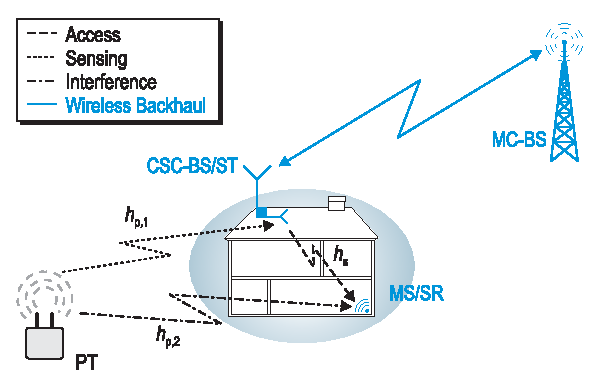
\includegraphics[width = \figscalet]{figures/CR_Scenario_Interweave}
\caption{A cognitive small cell scenario demonstrating: (i) the interweave paradigm, (ii) the associated network elements, which constitute cognitive small cell-base station/secondary transmitter (CSC-BS/ST), mobile station/secondary receiver (MS/SR), macro cell-base station (MC-BS) and primary transmitter (PT), (iii) the interacting channels: sensing channel $(\hpo)$, access channel $(\hs)$ and interference channel $(\hpt)$.} 
\label{fig:scenario}
\vspace{-0.5cm}
\end{figure}
\begin{figure}[!t]
\centering
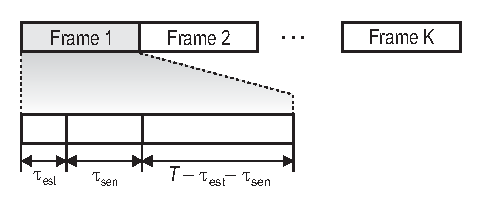
\includegraphics[width = \figscalet]{figures/Frame_Structure_grau}
\caption{\tc{An illustration of the frame structure for an interweave system depicting the estimation phase and the sensing phase for the sensing channel.}}
\label{fig:fs}
\vspace{-0.5cm}
\end{figure}

Complementing the analysis depicted in \cite{Liang08}, a slotted medium access for the IS is considered, according to which, the time axis is segmented into frames of length $T$. In order to incorporate channel estimation inside the frame, a frame structure that constitutes an estimation $\test$, a sensing $\tsen$ and data transmission $T - \tsen$ is employed, where $\test$ and $\tsen$ correspond to time intervals and $0 < \test \le \tsen < T$, refer to \figurename~{\ref{fig:fs}}\cite{Kaushik16}. From a deployment perspective, the estimated values of the interacting channels are required for determining the suitable sensing time (the duration of the sensing phase). In this regard, the sequence (estimation followed by sensing) depicted in \figurename~{\ref{fig:fs}} is followed.
As shown in the frame structure in \figurename~\ref{fig:fs}, the samples (particularly for the sensing channel) used for estimation can be used for sensing such that the time resources within the frame duration can be utilized efficiently. 
It is important to note that the estimates for the interference and access channels at the ST are acquired by means of a low-rate feedback channel from the SR to the ST.
%For small $T$ relative to the PUs' expected ON/OFF period, the requirement of the ST to be in alignment to PUs' medium access can be relaxed \cite{Tang11}.  
 
\subsection{Signal model}
%According to interweave system, ST considers a hypothesis testing to determine the presence ($\mathcal{H}_1$) or absence $(\mathcal{H}_0)$ of a signal transmitted by the PR. 
Based on the underlying hypothesis that depicts the presence $(\mathcal{H}_1)$ or absence ($\mathcal{H}_0$) of a PU signal, the discrete and real signal received at the ST is given by  
\begin{equation}
\yrcvd[n] = 
\begin{cases}
\hpo \cdot \xp[n] + w[n] & : \mathcal{H}_1 \\
w[n] & :\mathcal{H}_0
\end{cases},
\label{eq:sys_mod_p1s}
\end{equation}
where $\xp[n]$ corresponds to a discrete and real sample transmitted by the PT, $|\hpo|^2$ represents the power gain of the sensing channel for a given frame and $w[n]$ is additive white Gaussian noise at the ST. \tc{According to \cite{Liang08}, the signal $\xp[n]$ transmitted by the PUs} can be modelled as: (i) a phase shift keying modulated signal, or (ii) a Gaussian signal. 
%The signals that are prone to high inter-symbol interference or entail precoding can be modelled as Gaussian signals. 
In this paper, we focus our analysis on the latter case. As a result, the mean and the variance for the signal and the noise are determined as $\e{}{\xp[n]} = 0$, $\e{}{w[n]} = 0$, $\e{}{|\xp[n]|^2} = \spo$ and $\e{}{|w[n]|^2} = \npo$. The channel $\hpo$ is considered to be independent of $\xp[n]$ and $w[n]$, thus, $\yrcvd$ is also an independent and identically distributed (i.i.d.) random process. %The true received power is defined as
%\begin{align}
%\bprcvd = \e{}{|\yrcvd|^2}.
%\label{eq:tprcvd}
%\end{align}
%Based on (\ref{eq:tprcvd}), the received SNR at the ST is $\snrrcvd = \frac{\bprcvd}{\npo} - 1$.

Similar to (\ref{eq:sys_mod_p1s}), during data transmission, the discrete and real received signal at the SR conditioned on the detection probability ($\pd$) and false alarm probability ($\pfa$) is given by
\begin{equation}
\ys[n] = 
\begin{cases}
\hs \cdot \xs[n] + \hpt \cdot \xp[n] + w[n] & : 1 - \pd \\
\hs \cdot \xs[n] + w[n] & : 1 - \pfa
\end{cases},
\label{eq:sys_mod_ss}
\end{equation}
%and on the other side, the interference signal at the SR, transmitted by the PR follows 
%\begin{equation}
%\yp[n] = \sqrt{\gpt \cdot \apt}/ \cdot \xp[n] + w[n],
%\label{eq:sys_mod_p2s}
%\end{equation}
where $\xs[n]$ corresponds to discrete and real sample transmitted by the ST. Further, $|\hs|^2$ and $|\hpt|^2$ represent the power gains for the access and the interference channels, \tc{refer to} \figurename~\ref{fig:scenario}. 
%The %received powers at the SR from ST and PR are evaluated as $\ps = \s{\test \fsam}{|\ys[n]^2|}$ and $\pp = \s{\test \fsam}{|\yp[n]^2|}$ %Likewise (\ref{eq:sys_mod_p1s}), $\nap[n]$ and $\nas[n]$ represents circularly symmetric AWGN at PR and ST with zero mean and variance $\e{}{|\nap[n]|^2} = \npp$ and $\e{}{|\nas[n]|^2} = \nps$ correspondingly. Consider that $\ps$, $\ps$ and $\pp$ correspond to power for a given frame. 
%\subsubsection{Channel}
%, where $\bpp = \e{}{\pp}$ and $\bps = \e{}{\ps}$ correspond to their true value. Similar to ST-PR, the 
%received SNRs over the links ST-SR and PT-ST are $\snrs = \frac{\e{}{|\sqrt{\hs} \cdot \xs[n]|^2}}{ \npo}$ and $\snrp = \frac{\e{}{|\sqrt{\hpt} \cdot \xp[n]|^2}}{\npo}$.


\subsection{Channel fading}
%Following the frame structure in \figurename~\ref{fig:fs}, the alternating transmissions observe a different channel. 
Here, we characterize the channel gains $\phpo$, $\phpt$ and $\phs$ according to Nakagami-$m$ fading model. As a consequence, the power gains $\phpo$, $\phpt$ and $\phs$ follow a Gamma distribution \cite{Goldsmith05}, whose corresponding cumulative distribution functions are defined as
\begin{align}
\fphpo(x) = 1 - \Gamma\left(\mpo, \frac{\mpo x}{\bphpo}\right), \label{eq:dis_phpo}\\
\fphpt(x) = 1 - \Gamma\left(\mpt, \frac{\mpt x}{\bphpt}\right), \label{eq:dis_pght}\\  
\fphs(x) = 1 - \Gamma\left(\ms , \frac{\ms x}{\bphs}\right), \label{eq:dis_phs}
\end{align}
where $\mpo$, $\mpt$ and $\ms$ represent the Nakagami-$m$ parameter, whereas $\bphpo$, $\bphpt$, $\bphs$ are the expected values for channels $\phpo$, $\phpt$ and $\phs$, respectively, and $\Gamma(\cdot, \cdot)$ is a regularized upper-incomplete Gamma function \cite{abramo}.

\section{Theoretical Analysis} \label{sec:th_ana}

%%%%%%%%%%%%%%%%%%%%%%%%%%%%%%%%%%%%%%%%%%%%%%%%%%%%%%%%%%%%%%%%%%%%%%%%%%%%%%%%%%%%%%%%%
\subsection{Perfect Channel Knowledge (Conventional Approach)} \label{ssec:pce}
%%%%%%%%%%%%%%%%%%%%%%%%%%%%%%%%%%%%%%%%%%%%%%%%%%%%%%%%%%%%%%%%%%%%%%%%%%%%%%%%%%%%%%%%%
%\subsection{Estimation Model (EM)}
We first consider a scenario (also represented as ideal model) that precludes channel estimation, in other words, the ST assumes the perfect knowledge of the interacting channels. In this context, the ST encounters variations caused due to the channel fading only. These variations translate to the variations in the detection probability, more specifically those variations that do not meet the desired detection probability $(\pdd)$ results in harmful interference at the PR. To overcome this issue, \cite{Juarez11} proposed to employ an outage constraint over $\pd$, given as
\begin{align}
\p( \pd \le \pdd) \le \mpd, \label{eq:OC_i}
\end{align} 
where $\mpd$ represents the outage constraint. Using (\ref{eq:OC_i}), the ST is able to regulate harmful interference at the PR. As a result, a decision threshold ($\mu$) on the $\prcvd$ is obtained such that it satisfies the constraint defined (\ref{eq:OC_i}) for a certain value of $\tsen$. 

Besides the interference at the PR, the throughput at the SR is given by (\ref{eq:thr_i}), see top of the next page,
\begin{figure*}
\begin{align}
%\hspace{-8mm}
&\rs(\tsen) = \frac{T - \tsen}{T} \mathbb{E}_{\phs \phpt} \bigg[ \phz (1 - \pfa) \smash[b]{\overbrace{\log_2 \bigg( 1 + \frac{\phs \ptranst}{\npo} \bigg)}^{\cz}} + \pho (1 - \pd) \smash[b]{\overbrace{\log_2 \bigg( 1 + \frac{\phs \ptranst}{\phpt \ptranpt + \npo} \bigg)}^{\co}} \bigg] \label{eq:thr_i} 
\end{align}
\hrulefill
\vspace{-0.3cm}
\end{figure*}
where $\cz$ and $\co$ correspond to the data rate at the SR with and without interference from the PT. The signal to noise ratio for the links PT-ST and ST-SR are defined as: $\snrrcvd = \frac{\prcvd}{\npo} - 1$ and $\snrso = \frac{\phs \ptranst}{\npo}$, respectively, and the interference to noise ratio for the link PT-SR is given by $\snrpt = \frac{\prcvdsr}{\npo} - 1$. %It is worth noticing the fact that the authors in \cite{Juarez11} did not consider fading over the access and interference channels.
Since the detection probability and the secondary throughput are related through the sensing time, this relationship is exploited to determine a sensing-throughput tradeoff for the case with the perfect channel estimation. 
\begin{theorem} \label{th:th1}
\normalfont
Subject to an outage constraint on $\pd$, the sensing-throughput tradeoff that considers perfect channel estimation and random behaviour of the interacting channels, is given by  
\begin{align}
\trsoc(\ttsenoc) &= \maxi_{\tsen} \e{\pd, \phs, \phpt}{\rs(\tsen)}, \label{eq:STT_i} \\
\text{s.t.} & \text{ }\;  (\ref{eq:OC_i}) \nonumber \\ 
\text{s.t.} & \text{ }\;  0 < \tsen \le T. \nonumber
\end{align}
\end{theorem}  
\begin{remark} \label{rem:rem1}
\normalfont
It is worth noticing the fact the authors in \cite{Juarez11} applied channel fading only to the sensing channel. However, according to Problem \ref{th:th1}, we consider a more practical approach, whereby, we exercise channel fading also over the access and the interference channels. Since the perfect channel knowledge scenario is employed to benchmark the performance of those ISs that employ channel estimation (discussed later in Section \ref{ssec:ice}), we evaluate the parameters such as threshold (which is used for evaluating $\pd$ and $\pfa$) and the expected secondary throughput numerically\footnote{In our future work, we plan to obtain analytical expressions of the aforementioned parameters.}. 
\end{remark}

\subsection{Imperfect Channel Knowledge (Proposed Approach)} \label{ssec:ice}
Here, we consider the estimation of the interacting channels, where the interacting channels encounter channel fading. To employ channel estimation, an estimation time is allocated within the frame duration of the IS, cf. \figurename~\ref{fig:fs}. With this, the IS incorporates variations in the performance parameters ($\pd$ and $\rs$) due to the channel estimation and the channel fading. In order to facilitate the hardware complexity and the versatility to unknown PU signals (as proposed by the energy detector) requirements at the secondary system, we propose to employ received power-based estimation $(\eprcvd, \eprcvdsr)$ for the sensing and the interference channels at the ST and the SR and the pilot-based estimation $\ephs$ for the access channel. The characterization of the estimated parameters $\eprcvd$ and $\eprcvdsr$ for the sensing and the interference channel, and $\ephs$ for the access channel in terms of their cumulative distribution functions (cdfs), for the deterministic case, has been performed in \cite[cf. Section III-B]{Kaushik16}. The estimated parameters are used to estimate the performance parameters $\epd$, $\ecz$ and $\eco$, whose cdfs $\fpd$, $\fcz$ and $\fco$ are characterized in \cite[cf. Lemma 1, Lemma 2 and Lemma 3]{Kaushik16}. %In this paper, we extend the characterization of the sensing-throughput tradeoff by considering the random behaviour (or channel fading) of the interacting channels.  

In order to protect the PR against harmful interference, we employ an outage constraint that jointly captures the variations due to the channel estimation and the channel fading, defined as 
\begin{align}
\smash[b]{\underbrace{\mathbb{E}_{\phpo}{\smash[b]{\overbrace{[\p( \epd \le \pdd)]}^{\text{Channel Estimation}}}}}_{\text{Channel fading}}} &\le \mpd, \label{eq:OC_p} \\[-0.3em] \nonumber 
\end{align}
where $\e{\phpo}{\cdot}$ represents the expectation over the sensing channel. The variations due to the channel estimation only ($\p(\epd \le \pdd)$) are characterized in terms of cdf as \cite{Kaushik16}
\begin{align}
\fpd(x) = 1 - \Gamma \left( \frac{\tsen \fsam}{2}, \frac{\tsen \fsam}{4 \prcvd \Gamma^{-1}\left(x, \frac{\tsen \fsam}{2} \right)} \right), \label{eq:dis_pd}
\end{align}
where $\Gamma^{-1}(\cdot)$ represents the inverse function of regularized upper incomplete Gamma function. It is worth noticing that $\e{\phpo}{\cdot}$ in (\ref{eq:OC_p}) acts on $\prcvd$, as $\prcvd$ incorporates the variations due to fading in the sensing channel $\phpo$.

Next, we characterize the expression of the secondary throughput 
\begin{align}
\rs(\test, \tsen) &= \mathbb{E}_{\epd,\ecz,\eco,\phpo, \phs, \phpt} \bigg[ \frac{T - \tsen}{T} \times \nonumber \\ & \bigg( \phz (1 - \pfa) \ecz + \pho (1 -\epd) \eco \bigg) \bigg] \label{eq:thr_p}
\end{align}
where $\e{\epd,\ecz,\eco,\phpo, \phs, \phpt}{\cdot}$ corresponds to an expectation over the estimated parameters $\left( \epd, \ecz, \eco \right)$ and the channel fading $\left( \phpo, \phs, \phpt \right)$. Please note that the random behaviour of the interacting channels due to the fading is included in the estimated system parameters $\epd$, $\ecz$ and $\eco$, refer to (\ref{eq:thr_i}).

\begin{theorem} \label{th:th2}
\normalfont
Subject to an outage constraint on $\epd$, the sensing-throughput tradeoff for the IS that considers imperfect channel estimation and random behaviour of the interacting channels, is given by  
\begin{align}
\trsoc(\ttest, \ttsen) &= \maxi_{\tc{\test}, \tsen} \e{\epd, \ecz, \eco, \phpo, \phs, \phpt}{\rs(\test, \tsen)}, \nonumber \\ 
\text{s.t.} & \text{ }  (\ref{eq:OC_p}),  \\
\tc{\text{s.t.}} & \text{ }  \tc{0 < \test \le \tsen \le T.} \nonumber
\end{align}
\end{theorem} 
%In this regard, we analyze the performance of IS based on this constraint. 
%where $\mpd$ represents the outage constraint.  
%\subsubsection*{Methodology of analysis}

\begin{IEEEproof} 
In order to solve the constrained optimization problem, the following approach is considered. We first exploit the underlying constraint (\ref{eq:OC_p}) to determine the decision threshold $\mu$. Since it is complicated to obtain a closed form expression of $\mu$, in this regard, we obtain its value numerically. 

Using $\mu$ to determine $\e{\epd}{\epd}$ and $\pfa$ and evaluating an expectation over $\epd, \ecz, \eco, \phpo, \phs, \phpt$, we determine the expected secondary throughput as function of estimation and sensing time. Finally, this function is used to determine the suitable estimation time ($\ttest$) and sensing time ($\ttsen$).
\end{IEEEproof} 
\tc{In contrast to the ideal model (refer to Problem \ref{th:th1}), the sensing-throughput tradeoff investigated by the proposed approach (refer to Problem \ref{th:th2}) incorporates the imperfect channel knowledge. In this context, the performance characterization considered by the proposed framework is closer to the realistic situations.} 


\begin{remark} \label{rem:rem2}
%Subsequently, following the variation of optimum expected throughput $\trs(\test,\ttsen)$ (optimized over the sensing time) against the estimation time, 
\normalfont
Based on the expression $\rs(\test, \tsen)$ computed by the estimation model (referred as the proposed approach), we establish a fundamental relation between estimation time, sensing time and achievable throughput, this relationship is characterized as \textit{estimation-sensing-throughput tradeoff}. Based on this tradeoff, we determine a suitable estimation $\test = \ttest$ and a sensing time $\tsen = \ttsen$ that attains a maximum achievable throughput $\trs(\ttest,\ttsen)$ for the IS.  
\end{remark}

%%%%%%%%%%%%%%%%%%%%%%%%%%%%%%%%%%%%%%%%%%%%%%%%%%%%%%%%%%%%%%%%%%%%%%%%%%%%%%%%%%%%%%%%%
\section{Numerical Results} \label{sec:num_ana}
%%%%%%%%%%%%%%%%%%%%%%%%%%%%%%%%%%%%%%%%%%%%%%%%%%%%%%%%%%%%%%%%%%%%%%%%%%%%%%%%%%%%%%%%%
Here, we analyze the performance of the IS based on the proposed approach. To accomplish this: (i) we perform simulations to validate the expressions obtained in (\ref{eq:OC_p}) and (\ref{eq:thr_p}), (ii) we consider the ideal model to benchmark and evaluate the performance loss. %, (iii) we establish mathematical justification to the considered approximations. 
Although the expressions derived using our sensing-throughput analysis are general and applicable to all CR systems, the parameters are selected in such a way that they closely relate to the deployment scenario described in \figurename~{\ref{fig:scenario}. Unless stated explicitly, the choice of the parameters $\fsam = \SI{1}{MHz}$, $\bphpo, \bphpt = \SI{-100}{dB}$, $\bphs = \SI{-80}{dB}$, $T = \SI{100}{ms}$, $\pdd = 0.9$, $\mpd = 0.05$, $\npo = \SI{-100}{dBm}$, $\snrrcvd = \SI{0}{dB}$, $\snrpt = \SI{0}{dB}$, $\snrso = \SI{10}{dB}$, $\spo = \ptranpt = \SI{0}{dBm}$, $\ptranst = -\SI{10}{dBm}$, $\pho = 1 - \phz = 0.2$, $\test = \SI{1}{ms}$ and $\Ks =  10$ (number of pilot symbols used for pilot-based channel estimation) is considered for the analysis. In addition, we investigate the performance of the IS under the following fading scenarios : (i) severe fading $m = 1$ (Rayleigh fading), and (ii) mild fading $m = 1.5$. 
 
%\begin{table}
%%\vspace{-0.4cm}
%\renewcommand{\arraystretch}{1.2}
%\caption{Parameters for Numerical Analysis}
%%\vspace{-0.6cm}
%\label{tb:tb2}
%\centering
%\scriptsize{
%\begin{tabular}{c||c}
%\hline
%\bfseries Parameter & \bfseries Value \\
%\hline\hline
%$\fsam$  & $\SI{1}{MHz}$ \\ \hline
%$\hpo, \hpt$ & $\SI{-100}{dB}$ \\ \hline
%$\hs$ & $\SI{-80}{dB}$ \\ \hline 
%$T$ & $\SI{100}{ms}$ \\ \hline 
%$\pdd$ & 0.9, \\ \hline 
%$\mpd$ & $0.05$ \\ \hline 
%$\npo$ & $\SI{-100}{dBm}$ \\ \hline
%$\snrrcvd$ & $\SI{-10}{dB}$ \\ \hline
%$\snrpt$ & $\SI{-10}{dB}$ \\ \hline
%$\snrso$ & $\SI{10}{dB}$ \\ \hline
%$\spo = \ptranpt$ & $-\SI{10}{dBm}$ \\ \hline
%$\ptranst$ & $-\SI{10}{dBm}$ \\ \hline
%$\pho = 1 - \phz$ & 0.2 \\ \hline
%$\test$ & $\SI{1}{ms}$ \\ \hline
%$\Ks$ & 10 \\ \hline 
%\end{tabular}}
%\end{table}

%Here, we analyze the performance of the IS in terms of sensing-throughput tradoff subject to new interference constraints.  


\begin{figure}[!t]
\centering
%% Add psfrag entries
% This file is generated by the MATLAB m-file laprint.m. It can be included
% into LaTeX documents using the packages graphicx, color and psfrag.
% It is accompanied by a postscript file. A sample LaTeX file is:
%    \documentclass{article}\usepackage{graphicx,color,psfrag}
%    \begin{document}% This file is generated by the MATLAB m-file laprint.m. It can be included
% into LaTeX documents using the packages graphicx, color and psfrag.
% It is accompanied by a postscript file. A sample LaTeX file is:
%    \documentclass{article}\usepackage{graphicx,color,psfrag}
%    \begin{document}\input{fig_thr_sen_time_tradeoff_fading}\end{document}
% See http://www.mathworks.de/matlabcentral/fileexchange/loadFile.do?objectId=4638
% for recent versions of laprint.m.
%
% created by:           LaPrint version 3.16 (13.9.2004)
% created on:           12-Jul-2016 15:14:00
% eps bounding box:     16 cm x 12 cm
% comment:              
%
%\begin{psfrags}%
%\psfragscanon%
%
% text strings:
\psfrag{s05}[b][b]{\fontsize{8}{12}\fontseries{m}\mathversion{normal}\fontshape{n}\selectfont \color[rgb]{0,0,0}\setlength{\tabcolsep}{0pt}\begin{tabular}{c}$\rs(\test = \SI{1}{ms}, \tsen)$ [bits/sec/Hz]\end{tabular}}%
\psfrag{s06}[t][t]{\fontsize{8}{12}\fontseries{m}\mathversion{normal}\fontshape{n}\selectfont \color[rgb]{0,0,0}\setlength{\tabcolsep}{0pt}\begin{tabular}{c}$\tsen$ [ms]\end{tabular}}%
\psfrag{s10}[][]{\fontsize{10}{15}\fontseries{m}\mathversion{normal}\fontshape{n}\selectfont \color[rgb]{0,0,0}\setlength{\tabcolsep}{0pt}\begin{tabular}{c} \end{tabular}}%
\psfrag{s11}[][]{\fontsize{10}{15}\fontseries{m}\mathversion{normal}\fontshape{n}\selectfont \color[rgb]{0,0,0}\setlength{\tabcolsep}{0pt}\begin{tabular}{c} \end{tabular}}%
\psfrag{s12}[l][l]{\fontsize{8}{12}\fontseries{m}\mathversion{normal}\fontshape{n}\selectfont \color[rgb]{0,0,0}Simulated}%
\psfrag{s13}[l][l]{\fontsize{8}{12}\fontseries{m}\mathversion{normal}\fontshape{n}\selectfont \color[rgb]{0,0,0}IM, Problem 1}%
\psfrag{s14}[l][l]{\fontsize{8}{12}\fontseries{m}\mathversion{normal}\fontshape{n}\selectfont \color[rgb]{0,0,0}EM, Problem 2}%
\psfrag{s15}[l][l]{\fontsize{8}{12}\fontseries{m}\mathversion{normal}\fontshape{n}\selectfont \color[rgb]{0,0,0}$\trs(\test,\ttsen)$}%
\psfrag{s16}[l][l]{\fontsize{8}{12}\fontseries{m}\mathversion{normal}\fontshape{n}\selectfont \color[rgb]{0,0,0}Simulated}%
%
% axes font properties:
\fontsize{8}{12}\fontseries{m}\mathversion{normal}%
\fontshape{n}\selectfont%
%
% xticklabels:
\psfrag{x01}[t][t]{0}%
\psfrag{x02}[t][t]{5}%
\psfrag{x03}[t][t]{10}%
\psfrag{x04}[t][t]{15}%
%
% yticklabels:
\psfrag{v01}[r][r]{0}%
\psfrag{v02}[r][r]{0.5}%
\psfrag{v03}[r][r]{1}%
\psfrag{v04}[r][r]{1.5}%
\psfrag{v05}[r][r]{2}%
%
% Figure:
%\resizebox{8cm}{!}{\includegraphics{fig_thr_sen_time_tradeoff_fading.eps}}%
%\end{psfrags}%
%
% End fig_thr_sen_time_tradeoff_fading.tex
\end{document}
% See http://www.mathworks.de/matlabcentral/fileexchange/loadFile.do?objectId=4638
% for recent versions of laprint.m.
%
% created by:           LaPrint version 3.16 (13.9.2004)
% created on:           12-Jul-2016 15:14:00
% eps bounding box:     16 cm x 12 cm
% comment:              
%
%\begin{psfrags}%
%\psfragscanon%
%
% text strings:
\psfrag{s05}[b][b]{\fontsize{8}{12}\fontseries{m}\mathversion{normal}\fontshape{n}\selectfont \color[rgb]{0,0,0}\setlength{\tabcolsep}{0pt}\begin{tabular}{c}$\rs(\test = \SI{1}{ms}, \tsen)$ [bits/sec/Hz]\end{tabular}}%
\psfrag{s06}[t][t]{\fontsize{8}{12}\fontseries{m}\mathversion{normal}\fontshape{n}\selectfont \color[rgb]{0,0,0}\setlength{\tabcolsep}{0pt}\begin{tabular}{c}$\tsen$ [ms]\end{tabular}}%
\psfrag{s10}[][]{\fontsize{10}{15}\fontseries{m}\mathversion{normal}\fontshape{n}\selectfont \color[rgb]{0,0,0}\setlength{\tabcolsep}{0pt}\begin{tabular}{c} \end{tabular}}%
\psfrag{s11}[][]{\fontsize{10}{15}\fontseries{m}\mathversion{normal}\fontshape{n}\selectfont \color[rgb]{0,0,0}\setlength{\tabcolsep}{0pt}\begin{tabular}{c} \end{tabular}}%
\psfrag{s12}[l][l]{\fontsize{8}{12}\fontseries{m}\mathversion{normal}\fontshape{n}\selectfont \color[rgb]{0,0,0}Simulated}%
\psfrag{s13}[l][l]{\fontsize{8}{12}\fontseries{m}\mathversion{normal}\fontshape{n}\selectfont \color[rgb]{0,0,0}IM, Problem 1}%
\psfrag{s14}[l][l]{\fontsize{8}{12}\fontseries{m}\mathversion{normal}\fontshape{n}\selectfont \color[rgb]{0,0,0}EM, Problem 2}%
\psfrag{s15}[l][l]{\fontsize{8}{12}\fontseries{m}\mathversion{normal}\fontshape{n}\selectfont \color[rgb]{0,0,0}$\trs(\test,\ttsen)$}%
\psfrag{s16}[l][l]{\fontsize{8}{12}\fontseries{m}\mathversion{normal}\fontshape{n}\selectfont \color[rgb]{0,0,0}Simulated}%
%
% axes font properties:
\fontsize{8}{12}\fontseries{m}\mathversion{normal}%
\fontshape{n}\selectfont%
%
% xticklabels:
\psfrag{x01}[t][t]{0}%
\psfrag{x02}[t][t]{5}%
\psfrag{x03}[t][t]{10}%
\psfrag{x04}[t][t]{15}%
%
% yticklabels:
\psfrag{v01}[r][r]{0}%
\psfrag{v02}[r][r]{0.5}%
\psfrag{v03}[r][r]{1}%
\psfrag{v04}[r][r]{1.5}%
\psfrag{v05}[r][r]{2}%
%
% Figure:
%\resizebox{8cm}{!}{\includegraphics{fig_thr_sen_time_tradeoff_fading.eps}}%
%\end{psfrags}%
%
% End fig_thr_sen_time_tradeoff_fading.tex


\begin{tikzpicture}[scale=1]
\node[anchor=south west,inner sep=0] (image) at (0,0)
{
        \includegraphics[width= \figscale]{figures/fig_thr_sen_time_tradeoff_fading}
};
\begin{scope}[x={(image.south east)},y={(image.north west)}]

%\node[draw,fill=gray!10,font=\small] (senid) at (0.232,0.83) {$\trs$};
%\draw[black, ->] (senid.north) -- (0.232,0.93);
%\node[draw,fill=gray!10,font=\small] (senac) at (0.378,0.882) {$\trsac$};
%\draw[black, ->] (senac.east) -- (0.478,0.882);
%\node[draw,fill=gray!10,font=\small] (senoc) at (0.614,0.733) {$\trsoc$};
%\draw[black, ->] (senoc.north) -- (0.614,0.833);

\draw[black,thick,<->] (0.082,0.12) --  node[above, font=\small] {$\test$} (0.14,0.12);
\draw (0.82,0.8) arc(-160:160:0.007 and 0.021);
\node[draw, fill=gray!10, font=\scriptsize] (text4) at (0.72,0.74) {$m = 1$};
\draw[black, ->] (text4.east) -- (0.82,0.795);

\draw (0.38,0.907) arc(-160:160:0.007 and 0.021);
\node[draw, fill=gray!10, font=\scriptsize] (text5) at (0.27,0.847) {$m = 1.5$};
\draw[black, ->] (text5.east) -- (0.38,0.902);

%\draw[help lines,xstep=.1,ystep=.1] (0,0) grid (1,1);
%\foreach \x in {0,1,...,9} { \node [anchor=north] at (\x/10,0) {0.\x}; }
%\foreach \y in {0,1,...,9} { \node [anchor=east] at (0,\y/10) {0.\y}; }
\end{scope}
\end{tikzpicture}
\caption{\tc{Sensing-throughput tradeoff for the ideal model (IM) and estimation model (EM), $\snrrcvd = \SI{0}{dB}$, $\test = \SI{1}{ms}$ and $\mpd = 0.05$.}}
\label{fig:ST_gen}
\vspace{-0.4cm}
\end{figure}
First, we investigate the sensing-throughput tradeoff for a certain value of estimation time $\test = \SI{1}{ms}$, corresponding to the Ideal Model (IM) and Estimation Model (EM) that represent the perfect and the imperfect channel knowledge, respectively, refer to \figurename~\ref{fig:ST_gen}. It is observed that with the inclusion of $\test$ in the frame structure, the EM procures no throughput at the SR for the time interval $\test$. Furthermore, it is noticed that the suitable sensing time increases with the severity in the fading. To procure further insights, we consider the variation of other parameters on the performance of the IS. 


\begin{figure}[!t]

%% Add psfrag entries
% This file is generated by the MATLAB m-file laprint.m. It can be included
% into LaTeX documents using the packages graphicx, color and psfrag.
% It is accompanied by a postscript file. A sample LaTeX file is:
%    \documentclass{article}\usepackage{graphicx,color,psfrag}
%    \begin{document}% This file is generated by the MATLAB m-file laprint.m. It can be included
% into LaTeX documents using the packages graphicx, color and psfrag.
% It is accompanied by a postscript file. A sample LaTeX file is:
%    \documentclass{article}\usepackage{graphicx,color,psfrag}
%    \begin{document}\input{fig_opt_thr_vs_est_time_fading}\end{document}
% See http://www.mathworks.de/matlabcentral/fileexchange/loadFile.do?objectId=4638
% for recent versions of laprint.m.
%
% created by:           LaPrint version 3.16 (13.9.2004)
% created on:           12-Jul-2016 15:25:44
% eps bounding box:     16 cm x 12 cm
% comment:              
%
%\begin{psfrags}%
%\psfragscanon%
%
% text strings:
\psfrag{s05}[b][b]{\fontsize{8}{12}\fontseries{m}\mathversion{normal}\fontshape{n}\selectfont \color[rgb]{0,0,0}\setlength{\tabcolsep}{0pt}\begin{tabular}{c}$\rs(\test,\ttsen)$\end{tabular}}%
\psfrag{s06}[t][t]{\fontsize{8}{12}\fontseries{m}\mathversion{normal}\fontshape{n}\selectfont \color[rgb]{0,0,0}\setlength{\tabcolsep}{0pt}\begin{tabular}{c}$\test$ [ms]\end{tabular}}%
\psfrag{s10}[][]{\fontsize{10}{15}\fontseries{m}\mathversion{normal}\fontshape{n}\selectfont \color[rgb]{0,0,0}\setlength{\tabcolsep}{0pt}\begin{tabular}{c} \end{tabular}}%
\psfrag{s11}[][]{\fontsize{10}{15}\fontseries{m}\mathversion{normal}\fontshape{n}\selectfont \color[rgb]{0,0,0}\setlength{\tabcolsep}{0pt}\begin{tabular}{c} \end{tabular}}%
\psfrag{s12}[l][l]{\fontsize{8}{12}\fontseries{m}\mathversion{normal}\fontshape{n}\selectfont \color[rgb]{0,0,0}$\trs(\ttest,\ttsen)$}%
\psfrag{s13}[l][l]{\fontsize{8}{12}\fontseries{m}\mathversion{normal}\fontshape{n}\selectfont \color[rgb]{0,0,0}IM, Problem 1}%
\psfrag{s14}[l][l]{\fontsize{8}{12}\fontseries{m}\mathversion{normal}\fontshape{n}\selectfont \color[rgb]{0,0,0}EM, Problem 2}%
\psfrag{s15}[l][l]{\fontsize{8}{12}\fontseries{m}\mathversion{normal}\fontshape{n}\selectfont \color[rgb]{0,0,0}$\trs(\ttest,\ttsen)$}%
%
% axes font properties:
\fontsize{8}{12}\fontseries{m}\mathversion{normal}%
\fontshape{n}\selectfont%
%
% xticklabels:
\psfrag{x01}[t][t]{1}%
\psfrag{x02}[t][t]{2}%
\psfrag{x03}[t][t]{3}%
\psfrag{x04}[t][t]{4}%
\psfrag{x05}[t][t]{5}%
\psfrag{x06}[t][t]{6}%
\psfrag{x07}[t][t]{7}%
\psfrag{x08}[t][t]{8}%
\psfrag{x09}[t][t]{9}%
\psfrag{x10}[t][t]{10}%
\psfrag{x11}[t][t]{11}%
\psfrag{x12}[t][t]{12}%
%
% yticklabels:
\psfrag{v01}[r][r]{1}%
\psfrag{v02}[r][r]{1.2}%
\psfrag{v03}[r][r]{1.4}%
\psfrag{v04}[r][r]{1.6}%
\psfrag{v05}[r][r]{1.8}%
\psfrag{v06}[r][r]{2}%
\psfrag{v07}[r][r]{2.2}%
\psfrag{v08}[r][r]{2.4}%
%
% Figure:
%\resizebox{8cm}{!}{\includegraphics{fig_opt_thr_vs_est_time_fading.eps}}%
%\end{psfrags}%
%
% End fig_opt_thr_vs_est_time_fading.tex
\end{document}
% See http://www.mathworks.de/matlabcentral/fileexchange/loadFile.do?objectId=4638
% for recent versions of laprint.m.
%
% created by:           LaPrint version 3.16 (13.9.2004)
% created on:           12-Jul-2016 15:25:44
% eps bounding box:     16 cm x 12 cm
% comment:              
%
%\begin{psfrags}%
%\psfragscanon%
%
% text strings:
\psfrag{s05}[b][b]{\fontsize{8}{12}\fontseries{m}\mathversion{normal}\fontshape{n}\selectfont \color[rgb]{0,0,0}\setlength{\tabcolsep}{0pt}\begin{tabular}{c}$\rs(\test,\ttsen)$\end{tabular}}%
\psfrag{s06}[t][t]{\fontsize{8}{12}\fontseries{m}\mathversion{normal}\fontshape{n}\selectfont \color[rgb]{0,0,0}\setlength{\tabcolsep}{0pt}\begin{tabular}{c}$\test$ [ms]\end{tabular}}%
\psfrag{s10}[][]{\fontsize{10}{15}\fontseries{m}\mathversion{normal}\fontshape{n}\selectfont \color[rgb]{0,0,0}\setlength{\tabcolsep}{0pt}\begin{tabular}{c} \end{tabular}}%
\psfrag{s11}[][]{\fontsize{10}{15}\fontseries{m}\mathversion{normal}\fontshape{n}\selectfont \color[rgb]{0,0,0}\setlength{\tabcolsep}{0pt}\begin{tabular}{c} \end{tabular}}%
\psfrag{s12}[l][l]{\fontsize{8}{12}\fontseries{m}\mathversion{normal}\fontshape{n}\selectfont \color[rgb]{0,0,0}$\trs(\ttest,\ttsen)$}%
\psfrag{s13}[l][l]{\fontsize{8}{12}\fontseries{m}\mathversion{normal}\fontshape{n}\selectfont \color[rgb]{0,0,0}IM, Problem 1}%
\psfrag{s14}[l][l]{\fontsize{8}{12}\fontseries{m}\mathversion{normal}\fontshape{n}\selectfont \color[rgb]{0,0,0}EM, Problem 2}%
\psfrag{s15}[l][l]{\fontsize{8}{12}\fontseries{m}\mathversion{normal}\fontshape{n}\selectfont \color[rgb]{0,0,0}$\trs(\ttest,\ttsen)$}%
%
% axes font properties:
\fontsize{8}{12}\fontseries{m}\mathversion{normal}%
\fontshape{n}\selectfont%
%
% xticklabels:
\psfrag{x01}[t][t]{1}%
\psfrag{x02}[t][t]{2}%
\psfrag{x03}[t][t]{3}%
\psfrag{x04}[t][t]{4}%
\psfrag{x05}[t][t]{5}%
\psfrag{x06}[t][t]{6}%
\psfrag{x07}[t][t]{7}%
\psfrag{x08}[t][t]{8}%
\psfrag{x09}[t][t]{9}%
\psfrag{x10}[t][t]{10}%
\psfrag{x11}[t][t]{11}%
\psfrag{x12}[t][t]{12}%
%
% yticklabels:
\psfrag{v01}[r][r]{1}%
\psfrag{v02}[r][r]{1.2}%
\psfrag{v03}[r][r]{1.4}%
\psfrag{v04}[r][r]{1.6}%
\psfrag{v05}[r][r]{1.8}%
\psfrag{v06}[r][r]{2}%
\psfrag{v07}[r][r]{2.2}%
\psfrag{v08}[r][r]{2.4}%
%
% Figure:
%\resizebox{8cm}{!}{\includegraphics{fig_opt_thr_vs_est_time_fading.eps}}%
%\end{psfrags}%
%
% End fig_opt_thr_vs_est_time_fading.tex
 
\centering
\begin{tikzpicture}[scale=1]
\node[anchor=south west,inner sep=0] (image) at (0,0)
{
\includegraphics[width= \figscale]{figures/fig_opt_thr_vs_est_time_fading.eps} 
};
\begin{scope}[x={(image.south east)},y={(image.north west)}]


\draw (0.54,0.74) arc(-160:160:0.007 and 0.021);
\node[draw, fill=gray!10, font=\scriptsize] (text4) at (0.44,0.68) {$m = 1$};
\draw[black, ->] (text4.east) -- (0.54,0.735);

\draw (0.3,0.92) arc(-160:160:0.009 and 0.027);
\node[draw, fill=gray!10, font=\scriptsize] (text5) at (0.19,0.86) {$m = 1.5$};
\draw[black, ->] (text5.east) -- (0.302,0.913);


%\draw[black,->] (0.25,0.64) node[below =12.0,right=-20.0,  font=\scriptsize] {$\mpd \in \{0.05,0.10,0.15\}$} -- (0.18,0.84);
%%\draw[black,->] (0.25,0.6) node[below =12.0,right=-20.0,  font=\scriptsize] {$\mpd \in \{0.05,0.10,0.15\}$} -- (0.18,0.8);
%
%%\draw[help lines,xstep=.1,ystep=.1] (0,0) grid (1,1);
%%\foreach \x in {0,1,...,9} { \node [anchor=north] at (\x/10,0) {0.\x}; }
%%\foreach \y in {0,1,...,9} { \node [anchor=east] at (0,\y/10) {0.\y}; }
\end{scope}
\end{tikzpicture}

\caption{\tc{Estimation-sensing-throughput tradeoff for the outage constraint with $\snrrcvd = \SI{0}{dB}$, where the secondary throughput is maximized over the sensing time, $\trs(\test,\ttsen)$. Estimation-sensing-throughput tradeoff is utilized to determine a suitable estimation time $\ttest$ that maximizes the secondary throughput, $\trs(\ttest,\ttsen)$.}}
\label{fig:optT_test}
\vspace{-0.4cm}
\end{figure}

Upon maximizing the secondary throughput for a certain $\test$, we consider the variation of $\rs(\test, \ttsen)$ along the estimation time, refer to \figurename~\ref{fig:optT_test}. It is noticed that $\trs(\test, \ttsen)$ increases for low values of $\test$ and then decreases beyond $\ttest$. This can explained as follows, low $\test$ increases the variations in $\epd$, shifting the threshold to lower values, which subsequently increases $\pfa$, hence, degrading the achievable secondary throughput. Beyond $\ttest$, the variations are largely dominated by the channel fading, therefore, the IS observes no improvement by increasing $\test$. Moreover, it is observed that the mild fading scenarios are more sensitive to the performance degradation in terms of the secondary throughput. \figurename~\ref{fig:Pd_test} considers the variation of expected detection probability against $\test$. It is observed that, despite the variations due to the channel estimation and the channel fading considered by the EM, the outage constraint is satisfied for all values of $\test$.

\begin{figure}[!t]

%% Add psfrag entries
% This file is generated by the MATLAB m-file laprint.m. It can be included
% into LaTeX documents using the packages graphicx, color and psfrag.
% It is accompanied by a postscript file. A sample LaTeX file is:
%    \documentclass{article}\usepackage{graphicx,color,psfrag}
%    \begin{document}% This file is generated by the MATLAB m-file laprint.m. It can be included
% into LaTeX documents using the packages graphicx, color and psfrag.
% It is accompanied by a postscript file. A sample LaTeX file is:
%    \documentclass{article}\usepackage{graphicx,color,psfrag}
%    \begin{document}\input{fig_P_d_vs_est_time_fading}\end{document}
% See http://www.mathworks.de/matlabcentral/fileexchange/loadFile.do?objectId=4638
% for recent versions of laprint.m.
%
% created by:           LaPrint version 3.16 (13.9.2004)
% created on:           12-Jul-2016 15:25:47
% eps bounding box:     16 cm x 12 cm
% comment:              
%
%\begin{psfrags}%
%\psfragscanon%
%
% text strings:
\psfrag{s05}[b][b]{\fontsize{8}{12}\fontseries{m}\mathversion{normal}\fontshape{n}\selectfont \color[rgb]{0,0,0}\setlength{\tabcolsep}{0pt}\begin{tabular}{c}$\e{\epd, \phpo}{\epd}$\end{tabular}}%
\psfrag{s06}[t][t]{\fontsize{8}{12}\fontseries{m}\mathversion{normal}\fontshape{n}\selectfont \color[rgb]{0,0,0}\setlength{\tabcolsep}{0pt}\begin{tabular}{c}$\test$ [ms]\end{tabular}}%
\psfrag{s10}[][]{\fontsize{10}{15}\fontseries{m}\mathversion{normal}\fontshape{n}\selectfont \color[rgb]{0,0,0}\setlength{\tabcolsep}{0pt}\begin{tabular}{c} \end{tabular}}%
\psfrag{s11}[][]{\fontsize{10}{15}\fontseries{m}\mathversion{normal}\fontshape{n}\selectfont \color[rgb]{0,0,0}\setlength{\tabcolsep}{0pt}\begin{tabular}{c} \end{tabular}}%
\psfrag{s12}[l][l]{\fontsize{8}{12}\fontseries{m}\mathversion{normal}\fontshape{n}\selectfont \color[rgb]{0,0,0}EM, Problem 2}%
\psfrag{s13}[l][l]{\fontsize{8}{12}\fontseries{m}\mathversion{normal}\fontshape{n}\selectfont \color[rgb]{0,0,0}IM, Problem 1}%
\psfrag{s14}[l][l]{\fontsize{8}{12}\fontseries{m}\mathversion{normal}\fontshape{n}\selectfont \color[rgb]{0,0,0}EM, Problem 2}%
%
% axes font properties:
\fontsize{8}{12}\fontseries{m}\mathversion{normal}%
\fontshape{n}\selectfont%
%
% xticklabels:
\psfrag{x01}[t][t]{1}%
\psfrag{x02}[t][t]{2}%
\psfrag{x03}[t][t]{3}%
\psfrag{x04}[t][t]{4}%
\psfrag{x05}[t][t]{5}%
\psfrag{x06}[t][t]{6}%
\psfrag{x07}[t][t]{7}%
\psfrag{x08}[t][t]{8}%
\psfrag{x09}[t][t]{9}%
\psfrag{x10}[t][t]{10}%
\psfrag{x11}[t][t]{11}%
\psfrag{x12}[t][t]{12}%
%
% yticklabels:
\psfrag{v01}[r][r]{0.95}%
\psfrag{v02}[r][r]{0.96}%
\psfrag{v03}[r][r]{0.97}%
\psfrag{v04}[r][r]{0.98}%
%
% Figure:
%\resizebox{8cm}{!}{\includegraphics{fig_P_d_vs_est_time_fading.eps}}%
%\end{psfrags}%
%
% End fig_P_d_vs_est_time_fading.tex
\end{document}
% See http://www.mathworks.de/matlabcentral/fileexchange/loadFile.do?objectId=4638
% for recent versions of laprint.m.
%
% created by:           LaPrint version 3.16 (13.9.2004)
% created on:           12-Jul-2016 15:25:47
% eps bounding box:     16 cm x 12 cm
% comment:              
%
%\begin{psfrags}%
%\psfragscanon%
%
% text strings:
\psfrag{s05}[b][b]{\fontsize{8}{12}\fontseries{m}\mathversion{normal}\fontshape{n}\selectfont \color[rgb]{0,0,0}\setlength{\tabcolsep}{0pt}\begin{tabular}{c}$\e{\epd, \phpo}{\epd}$\end{tabular}}%
\psfrag{s06}[t][t]{\fontsize{8}{12}\fontseries{m}\mathversion{normal}\fontshape{n}\selectfont \color[rgb]{0,0,0}\setlength{\tabcolsep}{0pt}\begin{tabular}{c}$\test$ [ms]\end{tabular}}%
\psfrag{s10}[][]{\fontsize{10}{15}\fontseries{m}\mathversion{normal}\fontshape{n}\selectfont \color[rgb]{0,0,0}\setlength{\tabcolsep}{0pt}\begin{tabular}{c} \end{tabular}}%
\psfrag{s11}[][]{\fontsize{10}{15}\fontseries{m}\mathversion{normal}\fontshape{n}\selectfont \color[rgb]{0,0,0}\setlength{\tabcolsep}{0pt}\begin{tabular}{c} \end{tabular}}%
\psfrag{s12}[l][l]{\fontsize{8}{12}\fontseries{m}\mathversion{normal}\fontshape{n}\selectfont \color[rgb]{0,0,0}EM, Problem 2}%
\psfrag{s13}[l][l]{\fontsize{8}{12}\fontseries{m}\mathversion{normal}\fontshape{n}\selectfont \color[rgb]{0,0,0}IM, Problem 1}%
\psfrag{s14}[l][l]{\fontsize{8}{12}\fontseries{m}\mathversion{normal}\fontshape{n}\selectfont \color[rgb]{0,0,0}EM, Problem 2}%
%
% axes font properties:
\fontsize{8}{12}\fontseries{m}\mathversion{normal}%
\fontshape{n}\selectfont%
%
% xticklabels:
\psfrag{x01}[t][t]{1}%
\psfrag{x02}[t][t]{2}%
\psfrag{x03}[t][t]{3}%
\psfrag{x04}[t][t]{4}%
\psfrag{x05}[t][t]{5}%
\psfrag{x06}[t][t]{6}%
\psfrag{x07}[t][t]{7}%
\psfrag{x08}[t][t]{8}%
\psfrag{x09}[t][t]{9}%
\psfrag{x10}[t][t]{10}%
\psfrag{x11}[t][t]{11}%
\psfrag{x12}[t][t]{12}%
%
% yticklabels:
\psfrag{v01}[r][r]{0.95}%
\psfrag{v02}[r][r]{0.96}%
\psfrag{v03}[r][r]{0.97}%
\psfrag{v04}[r][r]{0.98}%
%
% Figure:
%\resizebox{8cm}{!}{\includegraphics{fig_P_d_vs_est_time_fading.eps}}%
%\end{psfrags}%
%
% End fig_P_d_vs_est_time_fading.tex

\centering
\begin{tikzpicture}[scale=1]
\node[anchor=south west,inner sep=0] (image) at (0,0)
{
\includegraphics[width= \figscale]{figures/fig_P_d_vs_est_time_fading.eps} 
};
\begin{scope}[x={(image.south east)},y={(image.north west)}]
\draw (0.64,0.632) arc(-160:160:0.0095 and 0.0285);
\node[draw, fill=gray!10, font=\scriptsize] (text4) at (0.54,0.572) {$m = 1$};
\draw[black, ->] (text4.east) -- (0.6425,0.624);

\draw (0.12,0.60) arc(-160:160:0.007 and 0.021);
\draw (0.12,0.685) arc(-160:160:0.007 and 0.021);
\node[draw, fill=gray!10, font=\scriptsize] (text5) at (0.34,0.8) {$m = 1.5$};
\draw[black, ->] (text5.west) -- (0.132,0.708);
\draw[black, ->] (text5.west) -- (0.132,0.623);


%\draw[black,->] (0.25,0.64) node[below =12.0,right=-20.0,  font=\scriptsize] {$\mpd \in \{0.05,0.10,0.15\}$} -- (0.18,0.84);
%%\draw[black,->] (0.25,0.6) node[below =12.0,right=-20.0,  font=\scriptsize] {$\mpd \in \{0.05,0.10,0.15\}$} -- (0.18,0.8);
%
%\draw[help lines,xstep=.1,ystep=.1] (0,0) grid (1,1);
%\foreach \x in {0,1,...,9} { \node [anchor=north] at (\x/10,0) {0.\x}; }
%\foreach \y in {0,1,...,9} { \node [anchor=east] at (0,\y/10) {0.\y}; }
\end{scope}
\end{tikzpicture}

\caption{Expected detection probability versus estimation time.}
\label{fig:Pd_test}
\vspace{-0.4cm}
\end{figure}

%\begin{figure}[!t]
%
%%% Add psfrag entries
%\input{figures/fig_P_f_vs_est_time_fading.tex}
%\centering
%\begin{tikzpicture}[scale=1]
%\node[anchor=south west,inner sep=0] (image) at (0,0)
%{
%\includegraphics[width= \figscale]{figures/fig_P_f_vs_est_time_fading.eps}
%};
%\begin{scope}[x={(image.south east)},y={(image.north west)}]
%%\draw[black,->] (0.25,0.64) node[below =12.0,right=-20.0,  font=\scriptsize] {$\mpd \in \{0.05,0.10,0.15\}$} -- (0.18,0.84);
%%%\draw[black,->] (0.25,0.6) node[below =12.0,right=-20.0,  font=\scriptsize] {$\mpd \in \{0.05,0.10,0.15\}$} -- (0.18,0.8);
%
%%%\draw[help lines,xstep=.1,ystep=.1] (0,0) grid (1,1);
%%%\foreach \x in {0,1,...,9} { \node [anchor=north] at (\x/10,0) {0.\x}; }
%%%\foreach \y in {0,1,...,9} { \node [anchor=east] at (0,\y/10) {0.\y}; }
%\end{scope}
%\end{tikzpicture}
%
%\caption{False alarm probability versus estimation time.}
%\label{fig:Pd_test}
%%%\vspace{-0.7cm}
%\end{figure}



\begin{figure}[!t]

%% Add psfrag entries
% This file is generated by the MATLAB m-file laprint.m. It can be included
% into LaTeX documents using the packages graphicx, color and psfrag.
% It is accompanied by a postscript file. A sample LaTeX file is:
%    \documentclass{article}\usepackage{graphicx,color,psfrag}
%    \begin{document}% This file is generated by the MATLAB m-file laprint.m. It can be included
% into LaTeX documents using the packages graphicx, color and psfrag.
% It is accompanied by a postscript file. A sample LaTeX file is:
%    \documentclass{article}\usepackage{graphicx,color,psfrag}
%    \begin{document}\input{fig_opt_thr_vs_m_fading}\end{document}
% See http://www.mathworks.de/matlabcentral/fileexchange/loadFile.do?objectId=4638
% for recent versions of laprint.m.
%
% created by:           LaPrint version 3.16 (13.9.2004)
% created on:           12-Jul-2016 15:15:47
% eps bounding box:     16 cm x 12 cm
% comment:              
%
%\begin{psfrags}%
%\psfragscanon%
%
% text strings:
\psfrag{s05}[b][b]{\fontsize{8}{12}\fontseries{m}\mathversion{normal}\fontshape{n}\selectfont \color[rgb]{0,0,0}\setlength{\tabcolsep}{0pt}\begin{tabular}{c}$\rs(\ttest, \ttsen)$ [bits/sec/Hz]\end{tabular}}%
\psfrag{s06}[t][t]{\fontsize{8}{12}\fontseries{m}\mathversion{normal}\fontshape{n}\selectfont \color[rgb]{0,0,0}\setlength{\tabcolsep}{0pt}\begin{tabular}{c}Nakagami-$m$ parameter\end{tabular}}%
\psfrag{s10}[][]{\fontsize{10}{15}\fontseries{m}\mathversion{normal}\fontshape{n}\selectfont \color[rgb]{0,0,0}\setlength{\tabcolsep}{0pt}\begin{tabular}{c} \end{tabular}}%
\psfrag{s11}[][]{\fontsize{10}{15}\fontseries{m}\mathversion{normal}\fontshape{n}\selectfont \color[rgb]{0,0,0}\setlength{\tabcolsep}{0pt}\begin{tabular}{c} \end{tabular}}%
\psfrag{s12}[l][l]{\fontsize{8}{12}\fontseries{m}\mathversion{normal}\fontshape{n}\selectfont \color[rgb]{0,0,0}Rayleigh}%
\psfrag{s13}[l][l]{\fontsize{8}{12}\fontseries{m}\mathversion{normal}\fontshape{n}\selectfont \color[rgb]{0,0,0}IM, Problem 1}%
\psfrag{s14}[l][l]{\fontsize{8}{12}\fontseries{m}\mathversion{normal}\fontshape{n}\selectfont \color[rgb]{0,0,0}EM, Problem 2}%
\psfrag{s15}[l][l]{\fontsize{8}{12}\fontseries{m}\mathversion{normal}\fontshape{n}\selectfont \color[rgb]{0,0,0}Rayleigh}%
%
% axes font properties:
\fontsize{8}{12}\fontseries{m}\mathversion{normal}%
\fontshape{n}\selectfont%
%
% xticklabels:
\psfrag{x01}[t][t]{$10^{0}$}%
\psfrag{x02}[t][t]{$10^{1}$}%
\psfrag{x03}[t][t]{$10^{2}$}%
%
% yticklabels:
\psfrag{v01}[r][r]{1.8}%
\psfrag{v02}[r][r]{2}%
\psfrag{v03}[r][r]{2.2}%
\psfrag{v04}[r][r]{2.4}%
\psfrag{v05}[r][r]{2.6}%
\psfrag{v06}[r][r]{2.8}%
%
% Figure:
%\resizebox{8cm}{!}{\includegraphics{fig_opt_thr_vs_m_fading.eps}}%
%\end{psfrags}%
%
% End fig_opt_thr_vs_m_fading.tex
\end{document}
% See http://www.mathworks.de/matlabcentral/fileexchange/loadFile.do?objectId=4638
% for recent versions of laprint.m.
%
% created by:           LaPrint version 3.16 (13.9.2004)
% created on:           12-Jul-2016 15:15:47
% eps bounding box:     16 cm x 12 cm
% comment:              
%
%\begin{psfrags}%
%\psfragscanon%
%
% text strings:
\psfrag{s05}[b][b]{\fontsize{8}{12}\fontseries{m}\mathversion{normal}\fontshape{n}\selectfont \color[rgb]{0,0,0}\setlength{\tabcolsep}{0pt}\begin{tabular}{c}$\rs(\ttest, \ttsen)$ [bits/sec/Hz]\end{tabular}}%
\psfrag{s06}[t][t]{\fontsize{8}{12}\fontseries{m}\mathversion{normal}\fontshape{n}\selectfont \color[rgb]{0,0,0}\setlength{\tabcolsep}{0pt}\begin{tabular}{c}Nakagami-$m$ parameter\end{tabular}}%
\psfrag{s10}[][]{\fontsize{10}{15}\fontseries{m}\mathversion{normal}\fontshape{n}\selectfont \color[rgb]{0,0,0}\setlength{\tabcolsep}{0pt}\begin{tabular}{c} \end{tabular}}%
\psfrag{s11}[][]{\fontsize{10}{15}\fontseries{m}\mathversion{normal}\fontshape{n}\selectfont \color[rgb]{0,0,0}\setlength{\tabcolsep}{0pt}\begin{tabular}{c} \end{tabular}}%
\psfrag{s12}[l][l]{\fontsize{8}{12}\fontseries{m}\mathversion{normal}\fontshape{n}\selectfont \color[rgb]{0,0,0}Rayleigh}%
\psfrag{s13}[l][l]{\fontsize{8}{12}\fontseries{m}\mathversion{normal}\fontshape{n}\selectfont \color[rgb]{0,0,0}IM, Problem 1}%
\psfrag{s14}[l][l]{\fontsize{8}{12}\fontseries{m}\mathversion{normal}\fontshape{n}\selectfont \color[rgb]{0,0,0}EM, Problem 2}%
\psfrag{s15}[l][l]{\fontsize{8}{12}\fontseries{m}\mathversion{normal}\fontshape{n}\selectfont \color[rgb]{0,0,0}Rayleigh}%
%
% axes font properties:
\fontsize{8}{12}\fontseries{m}\mathversion{normal}%
\fontshape{n}\selectfont%
%
% xticklabels:
\psfrag{x01}[t][t]{$10^{0}$}%
\psfrag{x02}[t][t]{$10^{1}$}%
\psfrag{x03}[t][t]{$10^{2}$}%
%
% yticklabels:
\psfrag{v01}[r][r]{1.8}%
\psfrag{v02}[r][r]{2}%
\psfrag{v03}[r][r]{2.2}%
\psfrag{v04}[r][r]{2.4}%
\psfrag{v05}[r][r]{2.6}%
\psfrag{v06}[r][r]{2.8}%
%
% Figure:
%\resizebox{8cm}{!}{\includegraphics{fig_opt_thr_vs_m_fading.eps}}%
%\end{psfrags}%
%
% End fig_opt_thr_vs_m_fading.tex

\centering
\begin{tikzpicture}[scale=1]
\node[anchor=south west,inner sep=0] (image) at (0,0)
{
\includegraphics[width= \figscale]{figures/fig_opt_thr_vs_m_fading.eps}
};
\begin{scope}[x={(image.south east)},y={(image.north west)}]
%\draw[black,->] (0.25,0.64) node[below =12.0,right=-20.0,  font=\scriptsize] {$\mpd \in \{0.05,0.10,0.15\}$} -- (0.18,0.84);
%%\draw[black,->] (0.25,0.6) node[below =12.0,right=-20.0,  font=\scriptsize] {$\mpd \in \{0.05,0.10,0.15\}$} -- (0.18,0.8);
%
%%\draw[help lines,xstep=.1,ystep=.1] (0,0) grid (1,1);
%%\foreach \x in {0,1,...,9} { \node [anchor=north] at (\x/10,0) {0.\x}; }
%%\foreach \y in {0,1,...,9} { \node [anchor=east] at (0,\y/10) {0.\y}; }
\end{scope}
\end{tikzpicture}

\caption{Variation of the achievable throughput $R(\ttest, \ttsen)$ with Nakagami-$m$ parameter for $\snrrcvd = \SI{0}{dB}$.} 
\label{fig:optT_m}
\vspace{-0.7cm}
\end{figure}

Finally, we investigate the performance degradation in terms of achievable secondary throughput $\rs(\ttest, \ttsen)$ versus the Nakagami-$m$ parameter that accounts for severity in the fading, refer to \figurename~\ref{fig:optT_m}. While comparing the IM and the EM, it can be concluded that, for situations where the variations in the system are affected more due to the channel estimation as compared to the channel fading, a greater performance degradation is observed by the EM. 

%\begin{figure*}[!t]
%\centering
%\subfloat[]{
%% This file is generated by the MATLAB m-file laprint.m. It can be included
% into LaTeX documents using the packages graphicx, color and psfrag.
% It is accompanied by a postscript file. A sample LaTeX file is:
%    \documentclass{article}\usepackage{graphicx,color,psfrag}
%    \begin{document}% This file is generated by the MATLAB m-file laprint.m. It can be included
% into LaTeX documents using the packages graphicx, color and psfrag.
% It is accompanied by a postscript file. A sample LaTeX file is:
%    \documentclass{article}\usepackage{graphicx,color,psfrag}
%    \begin{document}\input{fig_P_d_vs_est_time_diff_mu_AWGN}\end{document}
% See http://www.mathworks.de/matlabcentral/fileexchange/loadFile.do?objectId=4638
% for recent versions of laprint.m.
%
% created by:           LaPrint version 3.16 (13.9.2004)
% created on:           10-Nov-2015 13:50:43
% eps bounding box:     16 cm x 12 cm
% comment:              
%
%\begin{psfrags}%
%\psfragscanon%
%
% text strings:
\psfrag{s05}[b][b]{\fontsize{8}{12}\fontseries{m}\mathversion{normal}\fontshape{n}\selectfont \color[rgb]{0,0,0}\setlength{\tabcolsep}{0pt}\begin{tabular}{c}$\e{\pd}{\pd}$\end{tabular}}%
\psfrag{s06}[t][t]{\fontsize{8}{12}\fontseries{m}\mathversion{normal}\fontshape{n}\selectfont \color[rgb]{0,0,0}\setlength{\tabcolsep}{0pt}\begin{tabular}{c}$\test$ [ms]\end{tabular}}%
\psfrag{s10}[][]{\fontsize{10}{15}\fontseries{m}\mathversion{normal}\fontshape{n}\selectfont \color[rgb]{0,0,0}\setlength{\tabcolsep}{0pt}\begin{tabular}{c} \end{tabular}}%
\psfrag{s11}[][]{\fontsize{10}{15}\fontseries{m}\mathversion{normal}\fontshape{n}\selectfont \color[rgb]{0,0,0}\setlength{\tabcolsep}{0pt}\begin{tabular}{c} \end{tabular}}%
\psfrag{s12}[l][l]{\fontsize{8}{12}\fontseries{m}\mathversion{normal}\fontshape{n}\selectfont \color[rgb]{0,0,0}Corollary 1}%
\psfrag{s13}[l][l]{\fontsize{8}{12}\fontseries{m}\mathversion{normal}\fontshape{n}\selectfont \color[rgb]{0,0,0}IM}%
\psfrag{s14}[l][l]{\fontsize{8}{12}\fontseries{m}\mathversion{normal}\fontshape{n}\selectfont \color[rgb]{0,0,0}EM-AC, Thm. 1}%
\psfrag{s15}[l][l]{\fontsize{8}{12}\fontseries{m}\mathversion{normal}\fontshape{n}\selectfont \color[rgb]{0,0,0}EM-OC, Thm. 2}%
\psfrag{s16}[l][l]{\fontsize{8}{12}\fontseries{m}\mathversion{normal}\fontshape{n}\selectfont \color[rgb]{0,0,0}Corollary 1}%
%
% axes font properties:
\fontsize{8}{12}\fontseries{m}\mathversion{normal}%
\fontshape{n}\selectfont%
%
% xticklabels:
\psfrag{x01}[t][t]{1}%
\psfrag{x02}[t][t]{2}%
\psfrag{x03}[t][t]{3}%
\psfrag{x04}[t][t]{4}%
\psfrag{x05}[t][t]{5}%
\psfrag{x06}[t][t]{6}%
\psfrag{x07}[t][t]{7}%
\psfrag{x08}[t][t]{8}%
\psfrag{x09}[t][t]{9}%
\psfrag{x10}[t][t]{10}%
%
% yticklabels:
\psfrag{v01}[r][r]{0.8}%
\psfrag{v02}[r][r]{0.82}%
\psfrag{v03}[r][r]{0.84}%
\psfrag{v04}[r][r]{0.86}%
\psfrag{v05}[r][r]{0.88}%
\psfrag{v06}[r][r]{0.9}%
\psfrag{v07}[r][r]{0.92}%
\psfrag{v08}[r][r]{0.94}%
\psfrag{v09}[r][r]{0.96}%
\psfrag{v10}[r][r]{0.98}%
\psfrag{v11}[r][r]{1}%
%
% Figure:
%\resizebox{8cm}{!}{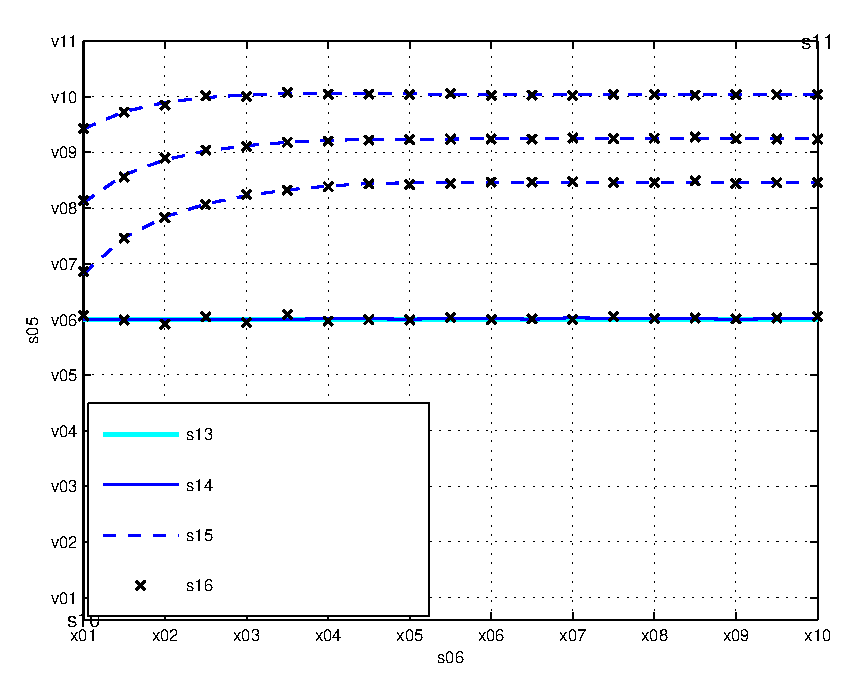
\includegraphics{fig_P_d_vs_est_time_diff_mu_AWGN.eps}}%
%\end{psfrags}%
%
% End fig_P_d_vs_est_time_diff_mu_AWGN.tex
\end{document}
% See http://www.mathworks.de/matlabcentral/fileexchange/loadFile.do?objectId=4638
% for recent versions of laprint.m.
%
% created by:           LaPrint version 3.16 (13.9.2004)
% created on:           10-Nov-2015 13:50:43
% eps bounding box:     16 cm x 12 cm
% comment:              
%
%\begin{psfrags}%
%\psfragscanon%
%
% text strings:
\psfrag{s05}[b][b]{\fontsize{8}{12}\fontseries{m}\mathversion{normal}\fontshape{n}\selectfont \color[rgb]{0,0,0}\setlength{\tabcolsep}{0pt}\begin{tabular}{c}$\e{\pd}{\pd}$\end{tabular}}%
\psfrag{s06}[t][t]{\fontsize{8}{12}\fontseries{m}\mathversion{normal}\fontshape{n}\selectfont \color[rgb]{0,0,0}\setlength{\tabcolsep}{0pt}\begin{tabular}{c}$\test$ [ms]\end{tabular}}%
\psfrag{s10}[][]{\fontsize{10}{15}\fontseries{m}\mathversion{normal}\fontshape{n}\selectfont \color[rgb]{0,0,0}\setlength{\tabcolsep}{0pt}\begin{tabular}{c} \end{tabular}}%
\psfrag{s11}[][]{\fontsize{10}{15}\fontseries{m}\mathversion{normal}\fontshape{n}\selectfont \color[rgb]{0,0,0}\setlength{\tabcolsep}{0pt}\begin{tabular}{c} \end{tabular}}%
\psfrag{s12}[l][l]{\fontsize{8}{12}\fontseries{m}\mathversion{normal}\fontshape{n}\selectfont \color[rgb]{0,0,0}Corollary 1}%
\psfrag{s13}[l][l]{\fontsize{8}{12}\fontseries{m}\mathversion{normal}\fontshape{n}\selectfont \color[rgb]{0,0,0}IM}%
\psfrag{s14}[l][l]{\fontsize{8}{12}\fontseries{m}\mathversion{normal}\fontshape{n}\selectfont \color[rgb]{0,0,0}EM-AC, Thm. 1}%
\psfrag{s15}[l][l]{\fontsize{8}{12}\fontseries{m}\mathversion{normal}\fontshape{n}\selectfont \color[rgb]{0,0,0}EM-OC, Thm. 2}%
\psfrag{s16}[l][l]{\fontsize{8}{12}\fontseries{m}\mathversion{normal}\fontshape{n}\selectfont \color[rgb]{0,0,0}Corollary 1}%
%
% axes font properties:
\fontsize{8}{12}\fontseries{m}\mathversion{normal}%
\fontshape{n}\selectfont%
%
% xticklabels:
\psfrag{x01}[t][t]{1}%
\psfrag{x02}[t][t]{2}%
\psfrag{x03}[t][t]{3}%
\psfrag{x04}[t][t]{4}%
\psfrag{x05}[t][t]{5}%
\psfrag{x06}[t][t]{6}%
\psfrag{x07}[t][t]{7}%
\psfrag{x08}[t][t]{8}%
\psfrag{x09}[t][t]{9}%
\psfrag{x10}[t][t]{10}%
%
% yticklabels:
\psfrag{v01}[r][r]{0.8}%
\psfrag{v02}[r][r]{0.82}%
\psfrag{v03}[r][r]{0.84}%
\psfrag{v04}[r][r]{0.86}%
\psfrag{v05}[r][r]{0.88}%
\psfrag{v06}[r][r]{0.9}%
\psfrag{v07}[r][r]{0.92}%
\psfrag{v08}[r][r]{0.94}%
\psfrag{v09}[r][r]{0.96}%
\psfrag{v10}[r][r]{0.98}%
\psfrag{v11}[r][r]{1}%
%
% Figure:
%\resizebox{8cm}{!}{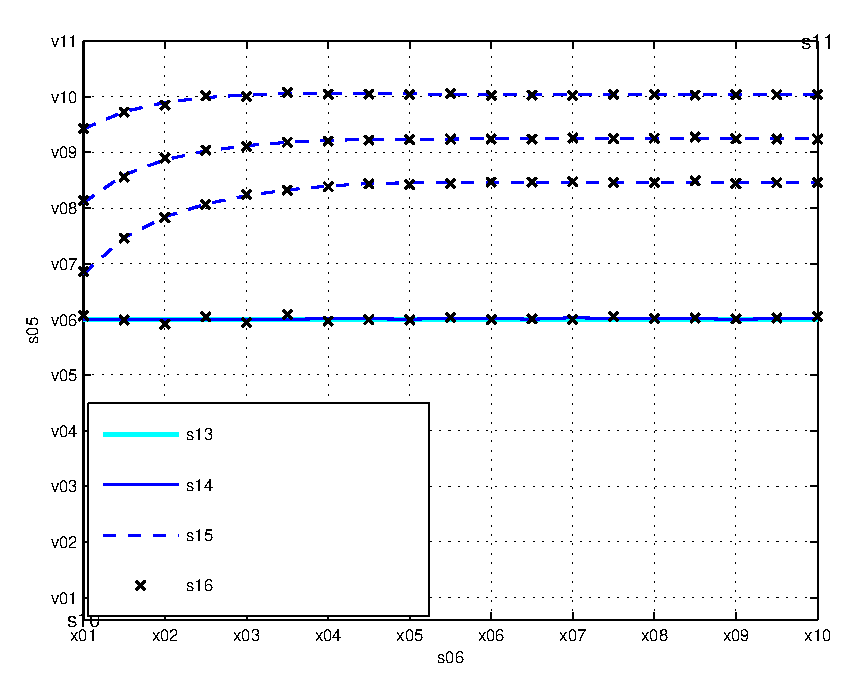
\includegraphics{fig_P_d_vs_est_time_diff_mu_AWGN.eps}}%
%\end{psfrags}%
%
% End fig_P_d_vs_est_time_diff_mu_AWGN.tex

%\begin{tikzpicture}[scale=1]
%\node[anchor=south west,inner sep=0] (image) at (0,0)
%{
%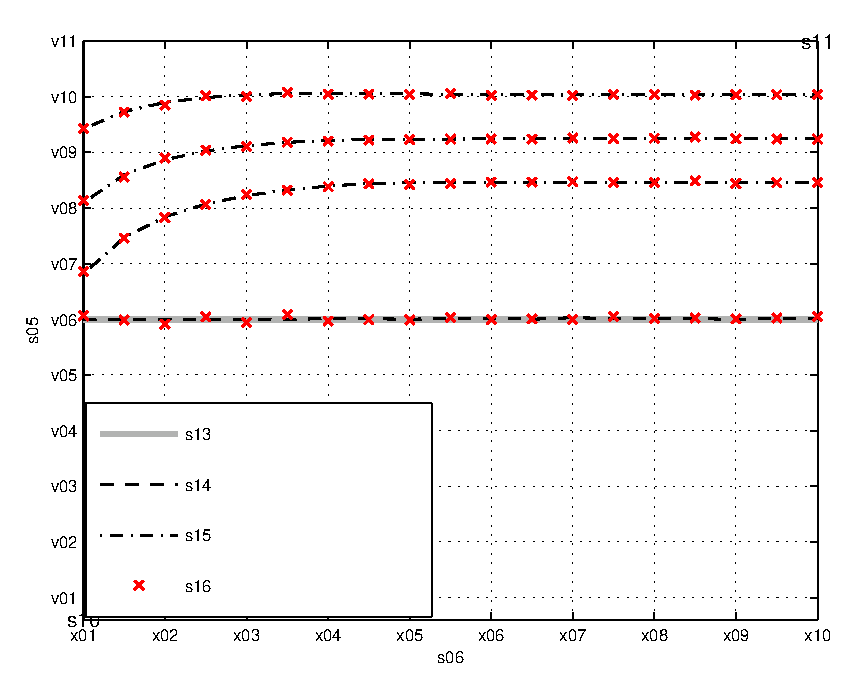
\includegraphics[width = \figscale]{figures/fig_P_d_vs_est_time_diff_mu_AWGN} 
%};
%\begin{scope}[x={(image.south east)},y={(image.north west)}]
%\draw[black,->] (0.25,0.68) node[below =10.0,right=-30.0,  font=\scriptsize] {$\mpd \in \{0.05,0.10,0.15\}$} -- (0.14,0.92);
%%\draw[help lines,xstep=.1,ystep=.1] (0,0) grid (1,1);
%%\foreach \x in {0,1,...,9} { \node [anchor=north] at (\x/10,0) {0.\x}; }
%%\foreach \y in {0,1,...,9} { \node [anchor=east] at (0,\y/10) {0.\y}; }
%\end{scope}
%\end{tikzpicture}
%
%\label{fig:pd_test}}
%\hfil
%\subfloat[]{
%% This file is generated by the MATLAB m-file laprint.m. It can be included
% into LaTeX documents using the packages graphicx, color and psfrag.
% It is accompanied by a postscript file. A sample LaTeX file is:
%    \documentclass{article}\usepackage{graphicx,color,psfrag}
%    \begin{document}% This file is generated by the MATLAB m-file laprint.m. It can be included
% into LaTeX documents using the packages graphicx, color and psfrag.
% It is accompanied by a postscript file. A sample LaTeX file is:
%    \documentclass{article}\usepackage{graphicx,color,psfrag}
%    \begin{document}\input{fig_P_f_vs_est_time_diff_mu_AWGN}\end{document}
% See http://www.mathworks.de/matlabcentral/fileexchange/loadFile.do?objectId=4638
% for recent versions of laprint.m.
%
% created by:           LaPrint version 3.16 (13.9.2004)
% created on:           12-Jul-2016 15:03:25
% eps bounding box:     16 cm x 12 cm
% comment:              
%
%\begin{psfrags}%
%\psfragscanon%
%
% text strings:
\psfrag{s05}[b][b]{\fontsize{8}{12}\fontseries{m}\mathversion{normal}\fontshape{n}\selectfont \color[rgb]{0,0,0}\setlength{\tabcolsep}{0pt}\begin{tabular}{c}$\pfa$\end{tabular}}%
\psfrag{s06}[t][t]{\fontsize{8}{12}\fontseries{m}\mathversion{normal}\fontshape{n}\selectfont \color[rgb]{0,0,0}\setlength{\tabcolsep}{0pt}\begin{tabular}{c}$\test$ = [ms]\end{tabular}}%
\psfrag{s10}[][]{\fontsize{10}{15}\fontseries{m}\mathversion{normal}\fontshape{n}\selectfont \color[rgb]{0,0,0}\setlength{\tabcolsep}{0pt}\begin{tabular}{c} \end{tabular}}%
\psfrag{s11}[][]{\fontsize{10}{15}\fontseries{m}\mathversion{normal}\fontshape{n}\selectfont \color[rgb]{0,0,0}\setlength{\tabcolsep}{0pt}\begin{tabular}{c} \end{tabular}}%
\psfrag{s12}[l][l]{\fontsize{8}{12}\fontseries{m}\mathversion{normal}\fontshape{n}\selectfont \color[rgb]{0,0,0}Corollary 1}%
\psfrag{s13}[l][l]{\fontsize{8}{12}\fontseries{m}\mathversion{normal}\fontshape{n}\selectfont \color[rgb]{0,0,0}IM}%
\psfrag{s14}[l][l]{\fontsize{8}{12}\fontseries{m}\mathversion{normal}\fontshape{n}\selectfont \color[rgb]{0,0,0}EM-AC, Problem 1}%
\psfrag{s15}[l][l]{\fontsize{8}{12}\fontseries{m}\mathversion{normal}\fontshape{n}\selectfont \color[rgb]{0,0,0}EM-OC, Problem 2}%
\psfrag{s16}[l][l]{\fontsize{8}{12}\fontseries{m}\mathversion{normal}\fontshape{n}\selectfont \color[rgb]{0,0,0}Corollary 1}%
%
% axes font properties:
\fontsize{8}{12}\fontseries{m}\mathversion{normal}%
\fontshape{n}\selectfont%
%
% xticklabels:
\psfrag{x01}[t][t]{1}%
\psfrag{x02}[t][t]{2}%
\psfrag{x03}[t][t]{3}%
\psfrag{x04}[t][t]{4}%
\psfrag{x05}[t][t]{5}%
\psfrag{x06}[t][t]{6}%
\psfrag{x07}[t][t]{7}%
\psfrag{x08}[t][t]{8}%
\psfrag{x09}[t][t]{9}%
\psfrag{x10}[t][t]{10}%
%
% yticklabels:
\psfrag{v01}[r][r]{$10^{-4}$}%
\psfrag{v02}[r][r]{$10^{-3}$}%
\psfrag{v03}[r][r]{$10^{-2}$}%
\psfrag{v04}[r][r]{$10^{-1}$}%
%
% Figure:
%\resizebox{8cm}{!}{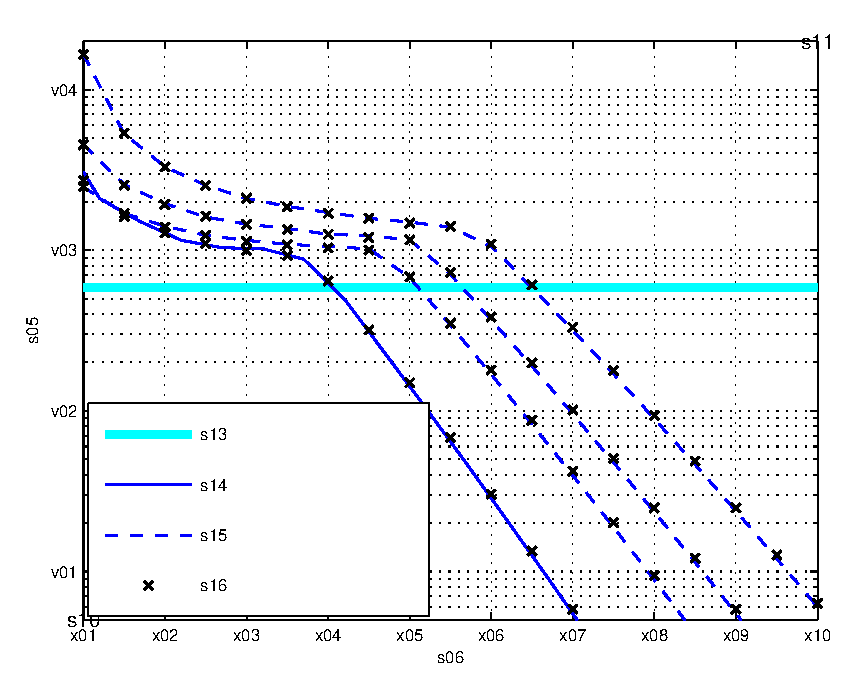
\includegraphics{fig_P_f_vs_est_time_diff_mu_AWGN.eps}}%
%\end{psfrags}%
%
% End fig_P_f_vs_est_time_diff_mu_AWGN.tex
\end{document}
% See http://www.mathworks.de/matlabcentral/fileexchange/loadFile.do?objectId=4638
% for recent versions of laprint.m.
%
% created by:           LaPrint version 3.16 (13.9.2004)
% created on:           12-Jul-2016 15:03:25
% eps bounding box:     16 cm x 12 cm
% comment:              
%
%\begin{psfrags}%
%\psfragscanon%
%
% text strings:
\psfrag{s05}[b][b]{\fontsize{8}{12}\fontseries{m}\mathversion{normal}\fontshape{n}\selectfont \color[rgb]{0,0,0}\setlength{\tabcolsep}{0pt}\begin{tabular}{c}$\pfa$\end{tabular}}%
\psfrag{s06}[t][t]{\fontsize{8}{12}\fontseries{m}\mathversion{normal}\fontshape{n}\selectfont \color[rgb]{0,0,0}\setlength{\tabcolsep}{0pt}\begin{tabular}{c}$\test$ = [ms]\end{tabular}}%
\psfrag{s10}[][]{\fontsize{10}{15}\fontseries{m}\mathversion{normal}\fontshape{n}\selectfont \color[rgb]{0,0,0}\setlength{\tabcolsep}{0pt}\begin{tabular}{c} \end{tabular}}%
\psfrag{s11}[][]{\fontsize{10}{15}\fontseries{m}\mathversion{normal}\fontshape{n}\selectfont \color[rgb]{0,0,0}\setlength{\tabcolsep}{0pt}\begin{tabular}{c} \end{tabular}}%
\psfrag{s12}[l][l]{\fontsize{8}{12}\fontseries{m}\mathversion{normal}\fontshape{n}\selectfont \color[rgb]{0,0,0}Corollary 1}%
\psfrag{s13}[l][l]{\fontsize{8}{12}\fontseries{m}\mathversion{normal}\fontshape{n}\selectfont \color[rgb]{0,0,0}IM}%
\psfrag{s14}[l][l]{\fontsize{8}{12}\fontseries{m}\mathversion{normal}\fontshape{n}\selectfont \color[rgb]{0,0,0}EM-AC, Problem 1}%
\psfrag{s15}[l][l]{\fontsize{8}{12}\fontseries{m}\mathversion{normal}\fontshape{n}\selectfont \color[rgb]{0,0,0}EM-OC, Problem 2}%
\psfrag{s16}[l][l]{\fontsize{8}{12}\fontseries{m}\mathversion{normal}\fontshape{n}\selectfont \color[rgb]{0,0,0}Corollary 1}%
%
% axes font properties:
\fontsize{8}{12}\fontseries{m}\mathversion{normal}%
\fontshape{n}\selectfont%
%
% xticklabels:
\psfrag{x01}[t][t]{1}%
\psfrag{x02}[t][t]{2}%
\psfrag{x03}[t][t]{3}%
\psfrag{x04}[t][t]{4}%
\psfrag{x05}[t][t]{5}%
\psfrag{x06}[t][t]{6}%
\psfrag{x07}[t][t]{7}%
\psfrag{x08}[t][t]{8}%
\psfrag{x09}[t][t]{9}%
\psfrag{x10}[t][t]{10}%
%
% yticklabels:
\psfrag{v01}[r][r]{$10^{-4}$}%
\psfrag{v02}[r][r]{$10^{-3}$}%
\psfrag{v03}[r][r]{$10^{-2}$}%
\psfrag{v04}[r][r]{$10^{-1}$}%
%
% Figure:
%\resizebox{8cm}{!}{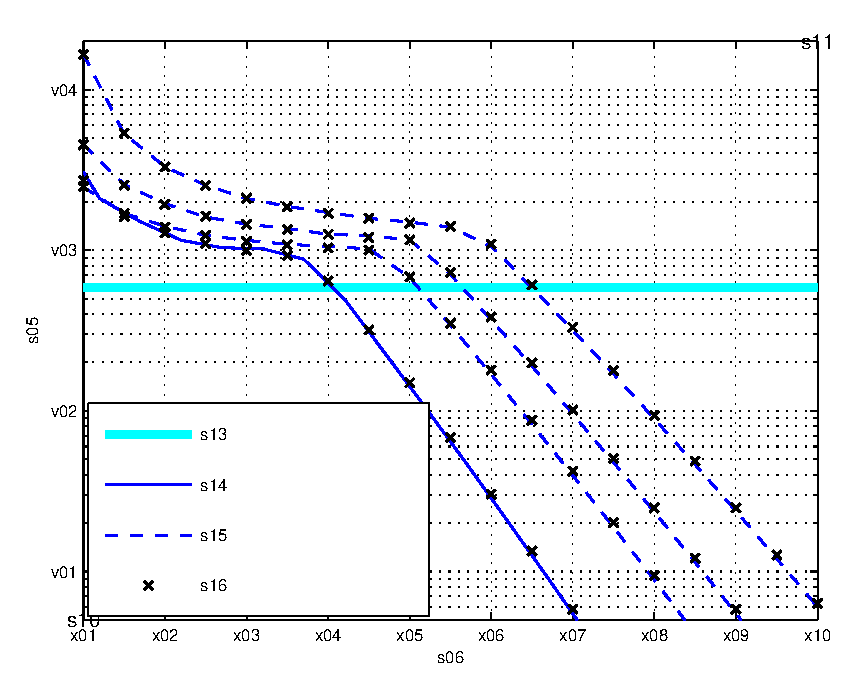
\includegraphics{fig_P_f_vs_est_time_diff_mu_AWGN.eps}}%
%\end{psfrags}%
%
% End fig_P_f_vs_est_time_diff_mu_AWGN.tex

%\begin{tikzpicture}[scale=1]
%\node[anchor=south west,inner sep=0] (image) at (0,0)
%{
%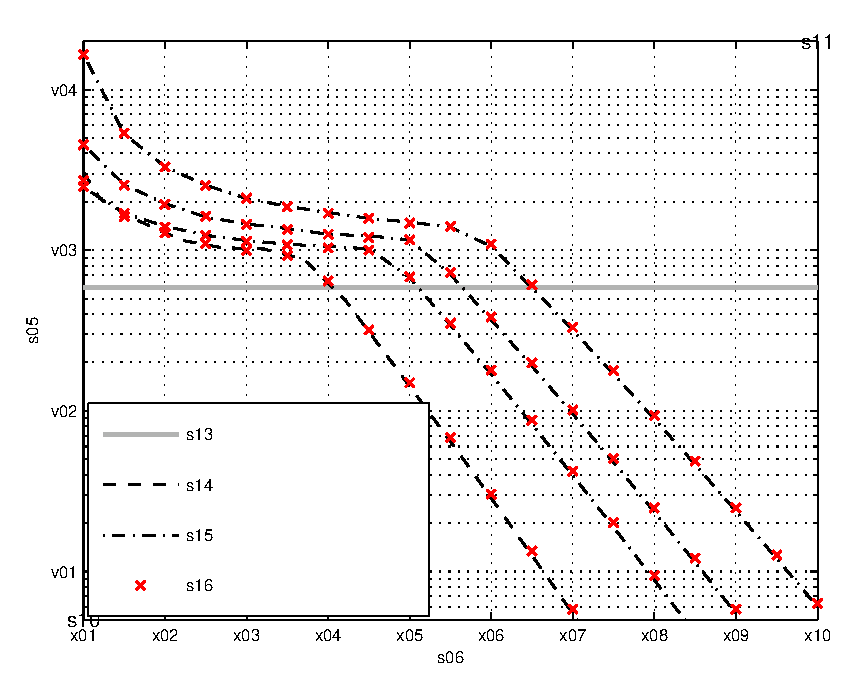
\includegraphics[width = \figscale]{figures/fig_P_f_vs_est_time_diff_mu_AWGN} 
%};
%\begin{scope}[x={(image.south east)},y={(image.north west)}]
%%\draw[black,->] (0.6,0.44) node[above=0.0,  font=\scriptsize] {$\mpd \in \{0.05,0.10,0.15\}$} -- (0.56,0.33);
%\draw[black,->] (0.75,0.47) node[above=0.0,  rotate=-50, font=\scriptsize] {$\mpd \in \{0.05,0.10,0.15\}$} -- (0.6,0.33);
%
%%\draw[help lines,xstep=.1,ystep=.1] (0,0) grid (1,1);
%%\foreach \x in {0,1,...,9} { \node [anchor=north] at (\x/10,0) {0.\x}; }
%%\foreach \y in {0,1,...,9} { \node [anchor=east] at (0,\y/10) {0.\y}; }
%\end{scope}
%\end{tikzpicture}
%
%\label{fig:pf_tsen}}
%\vspace{0.3cm}
%\caption{\tc{Variation of $\e{\pd}{\pd}$ and $\pfa$ versus the $\test$, where the secondary throughput is maximized over the sensing time, $\trs(\test,\ttsen)$. (a) Expected $\pd$ versus $\test$, (b) $\pfa$ versus $\test$.}} 
%\label{fig:ROC_test}
%%\vspace{-0.9cm}
%\end{figure*}

%Besides that, based on the previous discussion, it was analyzed that $\pfa$ accounts for a large contribution to the throughput. 




%%%%%%%%%%%%%%%%%%%%%%%%%%%%%%%%%%%%%%%%%%%%%%%%%%%%%%%%%%%%%%%%%%%%%%%%%%%%%%%%%%%%%%%%%
\section{Conclusion} \label{sec:conc}
%%%%%%%%%%%%%%%%%%%%%%%%%%%%%%%%%%%%%%%%%%%%%%%%%%%%%%%%%%%%%%%%%%%%%%%%%%%%%%%%%%%%%%%%%
Here, we characterized the performance of the ISs that incorporate imperfect knowledge of the interacting channels, considering these channels are subject to Nakagami-$m$ fading. An outage constraint that jointly captures the variations in the IS due to channel estimation and channel fading has been employed. Subject to this constraint, a sensing-throughput tradeoff that incorporates channel estimation and channel fading has been characterized, which yields a maximum secondary throughput at a suitable estimation and a sensing time. Finally, it has been concluded that the suitable choice of the estimation time is essential for controlling the performance degradation in terms of the achievable secondary throughput, particularly for scenarios that encounter less severe fading.  

 
%%%%%%%%%%%%%%%%%%%%%%%%%%%%%%%%%%%%%%%%%%%%%%%%%%%%%%%%%%%%%%%%%%%%%%%%%%%%%%%%%%%%%%%%%%
%\appendix[Moment Generating Function]
%%%%%%%%%%%%%%%%%%%%%%%%%%%%%%%%%%%%%%%%%%%%%%%%%%%%%%%%%%%%%%%%%%%%%%%%%%%%%%%%%%%%%%%%%%
%We intend to find the exact closed form expression of the moment generating function (mgf) of $\prcvd$ such that the received SNR $\gamma$ is subjected to small scale fading. To obtain its expression, we first consider the mgf of the received power $\prcvd$ for constant channel, that is $\gamma =$ constant. In this case, $\prcvd$ follows a non central chi-square distribution. The mgf of $\prcvd$ is given as   
%\begin{align}
%m_{\prcvd}(t) &= \frac{\exp\left( \frac{N \gamma t}{1- 2t}\right)}{(1 - 2t)^{N/2}}, 
%\text{where } 2t < N.    
%\label{eq:MGF_WOC} 
%\end{align}
%$N$ is the number of samples used for computing $\prcvd$. \\
%Considering Nakagami-$m$ fading, the probability density function (pdf) of $\gamma$ is given as
%\begin{equation}
%f(x) = \frac{\bar{\gamma}^{-m}}{\Gamma m}  x^{m-1} e^{-\frac{x}{\bar{\gamma}}}
%\label{eq:dis_ch}
%\end{equation}  
%where $\bar{\gamma}$ is the average received SNR and $m$ is the scaling factor. 
%
%Considering the case where $\gamma$ is distributed according to (\ref{eq:dis_ch}), the mgf for the $\prcvd$ is determined as  
%\begin{align}
%m'_{\prcvd}(t) &= \e{\gamma}{m_{\prcvd}(t)},  \nonumber \\ 
%	       &= \int\limits_{0}^{\infty} \frac{\bar{\gamma}^{-m}}{\Gamma m}  x^{m-1} e^{-\frac{x}{\bar{\gamma}}} \frac{\exp\left( \frac{N x t}{1- 2t}\right)}{(1 - 2t)^{N/2}} dx, \nonumber \\
%	       &= \frac{\bar{\gamma}^{-m}}{(1 - 2t)^{N/2}} \left( \frac{1}{\bar{\gamma}} - \frac{N t}{1 -2t} \right)^{-m}, \label{eq:MGF_WC} \\
%\quad & \text{where } {\frac{1}{\bar{\gamma}} - \frac{N t}{1 -2t} > 0} \text{ and } 2t < N. \nonumber
%\end{align}
%Based on (\ref{eq:MGF_WC}) the $n^{\text{th}}$ central moment can be evaluated as
%\begin{align}
%\psi_n &= \e{\prcvd}{ (\prcvd - \e{\prcvd}{\prcvd})^n}, \nonumber  \\ 
%\quad &= \lim_{t\to\infty} \frac{d^n}{dt^n} \log(m'_{\prcvd}(t)). 
%\label{eq:MGF_ME}
%\end{align}
%According to (\ref{eq:MGF_ME}), we obtain the expressions of the first four central moments as follows
%\begin{align}
%\psi_1 &= (1 + m \bar{\gamma}) \sigma^2, \label{eq:MGF_M1} \\ 
%\psi_2 &= \frac{1}{N} (2 + m \bar{\gamma} (4 + \bar{\gamma})) \sigma^4 , \label{eq:MGF_M2} \\ 
%\psi_3 &= \frac{2}{N^2} (4 + m \bar{\gamma} (12 + 6 \bar{\gamma} + \bar{\gamma}^2)) \sigma^6, \label{eq:MGF_M3}  \\ 
%\psi_4 &= \frac{6}{N^3} (8 + m \bar{\gamma} (32 + 24 \bar{\gamma} + 8 \bar{\gamma}^2 + \bar{\gamma}^3)) \sigma^8. \label{eq:MGF_M4}  
%\end{align}




\bibliographystyle{spmpsci}
\bibliography{IEEEfull,refs}

\end{document}
